% Provenance (never printed): see sources/outline_sources.md (Year 2: the vanished ocean;
% ophiolites; nappes; high-pressure rocks; foreland basins; reconstructing the history from
% maps, sections and geophysics). Units, ages and architecture after Schmid et al. (2004);
% Monte Cervino sheet notes (ISPRA 2016); Penrose definition as quoted by Coleman (1984);
% Zermatt-Saas ages Rubatto et al. (1998), Halama et al. (2020); Chenaillet Corno et al.
% (2023); Moho picks Michailos et al. (2023, Zenodo, CC BY 4.0); gravity Zahorec et al.
% (2021); Jura Lanza et al. (2022), Schori et al. (2015); shortening Rosenberg et al.
% (2021); Glarus thrust Herwegh et al. (2008); Molasse Krenmayr (1999), Garefalakis and
% Schlunegger (2018), Sinclair (1997); present uplift Champagnac et al. (2009). Figure data
% in figdata/bachelor-2/alps.py; exercise and problem values in the Book 4 scratch
% calculator calc/ch13.py.
\chapter{एक पर्वत-पट्टी की शारीरिकी: आल्प्स}\label{ch:b2:alpine-orogen}

मैटरहॉर्न का शिखर नाइस और गैब्रो से बना है जो कभी अपूलिया के किनारे के थे,
वह महाद्वीप जो एक लुप्त महासागर के अफ़्रीका वाले पक्ष पर स्थित था। उसके नीचे की ढलानें
उसी महासागर का तल हैं, यानी सर्पेंटिनाइट, गैब्रो और तकिया बेसाल्ट जो एक्लोजाइट में बदल गए, और
उनके नीचे, पड़ोसी मोंते रोसा में, यूरोप का किनारा स्थित है। इस ढेर में ऊपर चढ़ते हुए
व्यक्ति एक महाद्वीप से, एक महासागर से होकर, दूसरे महाद्वीप तक पहुँचता है। यह अध्याय आल्प्स को ऐसे ही एक ढेर के रूप में पढ़ता है: उसके टुकड़े कहाँ से आए, वे कैसे
चढ़ाए गए, चढ़ाव ने कितनी भूमि निगल ली, और भूभौतिकी नीचे क्या देखती है।
% ledger: ispra16:cervino, schmid04:apulia, schmid04:alpine-tethys

\begin{recall}
\textbf{पुस्तक 2 (उच्च माध्यमिक) से}: महाद्वीपीय टक्कर, सीवन, किसी परत का
लघुकरण (उसकी लंबाई का खोया अंश), उत्क्रम भ्रंश और प्रणोद। \textbf{पुस्तक 3 (स्नातक वर्ष
1) से}: भूवैज्ञानिक मानचित्र और अनुप्रस्थ काटें; सामान्य, उत्क्रम और अधिक्षेप भ्रंश, वलन और
वर्जेंस; निष्क्रिय किनारे; महासागरीय भूपर्पटी, तकिया-लावा और चादरी डाइक-संकुल;
सक्रिय किनारे और संचयी प्रिज़्म; समस्थिति, एयरी की जड़ और बूगेर विसंगति;
अवसादी द्रोणियों में गिनाई गई \omterm{def:b2:alpine-orogen:foreland}{अग्रभूमि द्रोणी}। \textbf{\cref{ch:b2:metamorphic-facies}
से}: नीलशिस्ट और एक्लोजाइट संलक्षणियाँ। \textbf{\cref{ch:b2:pt-paths}
से}: \omterm{def:b2:pt-paths:ptt}{P--T--t पथ}, \omterm{def:b2:pt-paths:exhumation}{उत्खनन-दरें} और \omterm{def:b2:pt-paths:uhp}{अति-उच्च-दाब
कायांतरण}।
\end{recall}

\begin{definition}[पर्वतजनक पट्टी]\label{def:b2:alpine-orogen:orogen}
\emph{पर्वतजनक पट्टी}\index{पर्वतजनक पट्टी} स्थलमंडल की वह पट्टी है जो दो प्लेटों के
अभिसरण से छोटी और मोटी हुई है, उसमें विरूपित और कायांतरित चट्टानों सहित; पर्वत-श्रेणी
उसकी सतही अभिव्यक्ति है, और नीचे की मोटी हुई भूपर्पटी उसकी जड़।
\end{definition}

\section{एक लुप्त महासागर}\label{sec:b2:alpine-orogen:tethys}

आल्प्स उन महासागरों के बंद होने को अंकित करते हैं जब अफ़्रीकी और यूरोपीय प्लेटें अभिसरित हो रही थीं।
मुख्य महासागर \emph{ऐल्पाइन टेथिस} है, जो दो शाखाओं से बना था। उसकी दक्षिणी शाखा,
पिएमोंट--लिगुरिया महासागर, मध्य जुरैसिक में अलग होने लगी, जब मध्य अटलांटिक
खुल रहा था: शुद्धगतिकी की दृष्टि से ऐल्पाइन टेथिस अटलांटिक के खुलने का भाग है, पूर्व के
टेथिसीय महासागरों के विपरीत। रेडियोलेराइट, यानी गहरे समुद्र के चट्टान बन चुके सिलिसियस ऊज़,
और ऐप्टिकस चूना-पत्थर प्रसार के आरंभ के बाद जमे, और वे आज भी उसके
अवशेषों की पहचान कराते हैं। एक संकरी उत्तरी शाखा, वालै महासागर, संभवतः सबसे आरंभिक
क्रिटेशस में खुली। दोनों के बीच महाद्वीप की एक पतली पट्टिका थी, ब्रियांसोनै पट्टिका, जो
पूर्व की ओर पतली होती जाती है और पूर्वी आल्प्स में अनुपस्थित है।
% ledger: schmid04:alpine-tethys

उत्तर में महासागर यूरोप के निष्क्रिय किनारे से घिरा था, जो पुस्तक 3 (स्नातक वर्ष 1) के दरार और
किनारों वाले अध्याय का विषय है। दक्षिण में \emph{अपूलिया} था: ऐल्पाइन टेथिस के दक्षिण और
अपेक्षाकृत युवा नियोटेथिस के उत्तर की सारी महाद्वीपीय भूमि, उस अग्रभूमि सहित
जो अब आल्प्स के दक्षिण में स्थित है। मैटरहॉर्न का शिखर उसी का एक टुकड़ा है।
% ledger: schmid04:apulia
नीचे का मानचित्र इस पट्टी और इस अध्याय के स्थानों को दर्शाता है।

\begin{omfigure}
\centering
% ledger: data:b4-etopo-alps, schmid04:windows, schmid04:foreland, ispra16:cervino
\begin{tikzpicture}
\begin{axis}[width=0.96\linewidth, height=0.74\linewidth, xmin=5, xmax=14, ymin=43.5,
  ymax=48.5, xlabel={देशांतर (\unit{\degree} E)}, ylabel={अक्षांश (\unit{\degree} N)},
  tick label style={font=\scriptsize}, label style={font=\small}, clip=true,
  xtick={5,6,...,14}, ytick={44,45,...,48}]
\addplot[omThm!35, line width=0.3pt] table[x=lon, y=lat] {figdata/out/bachelor-2-alps-c1000.dat};
\addplot[omThm!90!black, line width=0.45pt] table[x=lon, y=lat] {figdata/out/bachelor-2-alps-c2000.dat};
\addplot[blue!60!black, line width=0.5pt] table[x=lon, y=lat] {figdata/out/bachelor-2-alps-c0.dat};
\draw[red!70!black, line width=1pt] (axis cs:8,45.3) -- (axis cs:8,48.0);
\node[font=\scriptsize\bfseries, red!70!black, anchor=north west] at (axis cs:8.02,45.32) {A};
\node[font=\scriptsize\bfseries, red!70!black, anchor=south west] at (axis cs:8.02,47.98) {B};
\fill (axis cs:6.865,45.833) circle (1.3pt) node[font=\scriptsize, fill=white, fill opacity=0.85, text opacity=1, inner sep=1pt, anchor=north east] {मों ब्लां};
\fill (axis cs:7.659,45.976) circle (1.3pt) node[font=\scriptsize, fill=white, fill opacity=0.85, text opacity=1, inner sep=1pt, anchor=south east] {मैटरहॉर्न};
\node[font=\scriptsize\itshape, rotate=40] at (axis cs:6.35,46.85) {जूरा};
\node[font=\scriptsize\itshape] at (axis cs:9.35,47.65) {मोलास द्रोणी};
\node[font=\scriptsize\itshape] at (axis cs:10.0,45.05) {पो मैदान};
\node[font=\scriptsize\itshape, align=center, fill=white, fill opacity=0.8, text opacity=1, inner sep=1pt] at (axis cs:10.3,46.95) {एंगाडीन\\खिड़की};
\node[font=\scriptsize\itshape, align=center, fill=white, fill opacity=0.8, text opacity=1, inner sep=1pt] at (axis cs:12.6,47.25) {टाउअर्न\\खिड़की};
\node[font=\scriptsize\itshape] at (axis cs:8.6,43.85) {लिगुरियाई सागर};
\end{axis}
\end{tikzpicture}
\par\smallskip{\small ETOPO1 उच्चावच मॉडल से आल्प्स, जिसके नोड \qty{0.05}{\degree}
की दूरी पर हैं: \qty{1000}{m} (हल्की) और \qty{2000}{m} (गहरी) पर समोच्च रेखाएँ और तटरेखा।
इस ग्रिड का सबसे ऊँचा नोड \qty{3914}{m} है, मों ब्लां के निकट; शिखर इससे ऊँचे हैं,
क्योंकि ग्रिड-नोड एक कोष्ठिका का प्रतिचयन करता है, शिखर का नहीं। \qty{8}{\degree} E के अनुदिश रेखा A--B
अध्याय के अंतिम अनुभाग में खींची गई रूपरेखा है। लक्षणों के नाम हाथ से उनकी
अनुमानित स्थितियों पर रखे गए हैं।}
\end{omfigure}

जो महासागर लुप्त हो चुका है, उसे कैसे जाना जा सकता है? उसके तल के उन टुकड़ों से जो
क्षेपण से बच गए और पर्वत-पट्टी में फँस गए।

\begin{definition}[ओफ़ियोलाइट; पेनरोज़ ओफ़ियोलाइट अनुक्रम]\label{def:b2:alpine-orogen:ophiolite}
\emph{ओफ़ियोलाइट}\index{ओफ़ियोलाइट} मैफ़िक से अल्ट्रामैफ़िक चट्टानों का एक विशिष्ट समुच्चय है,
महासागरीय स्थलमंडल का एक टुकड़ा जो अब भूमि पर मिलता है। \emph{पेनरोज़ ओफ़ियोलाइट
अनुक्रम}\index{पेनरोज़ ओफ़ियोलाइट अनुक्रम} वह पूर्ण समुच्चय है जिसे 1972 में भूवैज्ञानिकों के एक
सम्मेलन ने परिभाषित किया; नीचे से ऊपर:
\begin{enumerate}
\item \omterm{def:b2:mantle-melting:peridotites}{हार्ज़बर्गाइट}, \omterm{def:b2:mantle-melting:peridotites}{लर्ज़ोलाइट} और \omterm{def:b2:mantle-melting:peridotites}{ड्यूनाइट} का एक अल्ट्रामैफ़िक संकुल, सामान्यतः
ठोस अवस्था में अर्जित विरूपण-गठन के साथ;
\item एक गैब्रोई संकुल, साधारणतः क्यूम्यूलस गठनों के साथ;
\item एक मैफ़िक चादरी डाइक-संकुल;
\item एक मैफ़िक ज्वालामुखीय संकुल, प्रायः तकिया-रूपी।
\end{enumerate}
\end{definition}
% ledger: coleman84:penrose

पेनरोज़ परिभाषा एक सर्वसम्मति थी, जिसकी आरंभ से ही आलोचना हुई, और जो अब भी सामान्यतः
स्वीकृत है। उसका अनुक्रम महासागरीय भूपर्पटी और ऊपरी प्रावार की वही परतें हैं जो पुस्तक 3
(स्नातक वर्ष 1) में मिलीं: तकिया-लावा, उनके नीचे चादरी \omterm{def:b2:magma-emplacement:bodies}{डाइक}, उनके नीचे गैब्रो, उसके नीचे प्रावार। फिर भी \omterm{def:b2:alpine-orogen:ophiolite}{ओफ़ियोलाइट}
औसत महासागर-तल नहीं हैं। अधिकांश वितलीय भूपर्पटी, यानी विस्तृत महासागरों की भूपर्पटी, क्षेपण
में खप जाती है; कोलमैन का तर्क था कि ऐल्पाइन और कॉर्डिलेरी पट्टियों के \omterm{def:b2:alpine-orogen:ophiolite}{ओफ़ियोलाइट}
मुख्यतः छोटी महासागरीय द्रोणियों के प्रसार केंद्रों पर या द्वीप-चापों के बीच बने, और कि
टेथिसीय \omterm{def:b2:alpine-orogen:ophiolite}{ओफ़ियोलाइट} वहाँ बने जहाँ महाद्वीपीय भूपर्पटी निष्क्रिय किनारों के अनुदिश तब तक पतली हुई जब तक एक छोटा
महासागर न खुल गया।
% ledger: coleman84:penrose, coleman84:settings

ऐल्पाइन \omterm{def:b2:alpine-orogen:ophiolite}{ओफ़ियोलाइट} उस चित्र में ठीक बैठते हैं। पिएमोंट--लिगुरिया महासागर से व्युत्पन्न इकाइयाँ
महासागरीय स्थलमंडल के और उस प्रावार के अवशेष हैं जो पतले हुए महाद्वीप के नीचे से
ऊपर लाया गया था, यानी उप-महाद्वीपीय प्रावार, और समुद्र-तल पर अनावृत हुआ।
पश्चिमी आल्प्स में शनाये पर, इनमें सबसे अच्छी तरह संरक्षित \omterm{def:b2:alpine-orogen:ophiolite}{ओफ़ियोलाइट} अनावृत
प्रावार, गैब्रो और तकिया बेसाल्टों का एक प्रसिद्ध अनुक्रम दिखाता है, बिना किसी अवसादी आवरण के।
नीचे का फ़ोटो उन्हें दिखाता है।
% ledger: schmid04:units, corno23:chenaillet

\begin{omfigure}
\centering
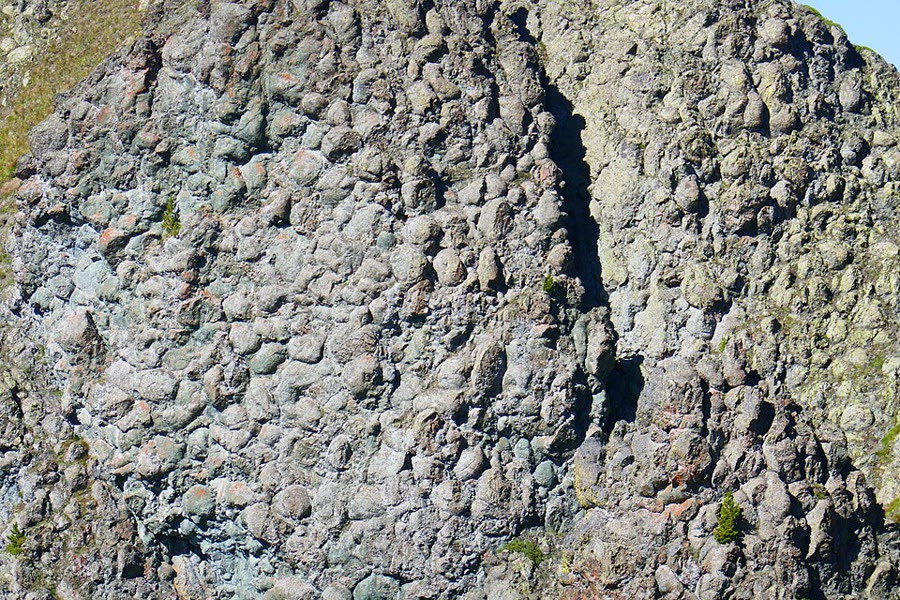
\includegraphics[width=0.66\linewidth]{images/book4/b2-13-pillow-lava.jpg}
\par\smallskip{\small शनाये \omterm{def:b2:alpine-orogen:ophiolite}{ओफ़ियोलाइट}, पश्चिमी आल्प्स, के तकिया-लावा: हर गोल
गद्दी बेसाल्ट का एक पिंड है जो पिएमोंट--लिगुरिया
महासागर के तल पर उद्गारित होकर ठंडा हुआ। फ़ोटो: Lionel Duchoiselle, CC BY-SA 3.0।}
\end{omfigure}

महासागर-तल का काल-निर्धारण वहाँ किया जा सकता है जहाँ उसके गैब्रो क्रिस्टलित हुए। मैटरहॉर्न के नीचे स्थित
त्सेरमाट--सास \omterm{def:b2:alpine-orogen:ophiolite}{ओफ़ियोलाइट} के दो मेटागैब्रो के ज़िरकॉन $164.0 \pm \qty{2.7}{Ma}$ और $163.5
\pm \qty{1.8}{Ma}$ देते हैं, और बेसाल्टों पर जमे मैंगनीज़-समृद्ध अवसाद अधिक से अधिक $161
\pm \qty{11}{Ma}$ पुराने हैं: पिएमोंट--लिगुरिया महासागर का तल जुरैसिक में,
लगभग \qty{164}{Myr} पहले, बन रहा था।
% ledger: rubatto98:zsf

\section{पहले एक महासागर का क्षेपण, फिर एक महाद्वीप का}\label{sec:b2:alpine-orogen:subduction}

महासागर क्षेपण से बंद होता है। फिर भी उसके तल का कुछ भाग किसी महाद्वीप के नीचे के बजाय
उसके ऊपर पहुँच जाता है, और कुछ महाद्वीप महासागर के पीछे-पीछे नीचे जाते हैं।

\begin{definition}[अधिरोहण; महाद्वीपीय क्षेपण]\label{def:b2:alpine-orogen:obduction}
\emph{अधिरोहण}\index{अधिरोहण} (ऑब्डक्शन) महासागरीय स्थलमंडल की एक पट्टिका का
किसी महाद्वीपीय किनारे पर स्थापन है, जिसमें \omterm{def:b2:alpine-orogen:ophiolite}{ओफ़ियोलाइट} महाद्वीप के ऊपर चढ़ जाता है। \emph{महाद्वीपीय
क्षेपण}\index{महाद्वीपीय क्षेपण} महाद्वीपीय स्थलमंडल का, उससे जुड़ी महासागरीय पट्टिका द्वारा खींचे जाकर,
किसी क्षेपण क्षेत्र में अवतरण है, जब उसके सामने का महासागर
खप चुका हो।
\end{definition}

\omterm{def:b2:alpine-orogen:obduction}{अधिरोहण} आल्प्स के दक्षिण-पूर्व में डिनारिडीज़ में हुआ: जुरैसिक वार्दार
महासागर के \omterm{def:b2:alpine-orogen:ophiolite}{ओफ़ियोलाइट}, जो स्वयं मध्य जुरैसिक आयु के हैं, उत्तर जुरैसिक में एक
संचयी कील पर और अपूलिया के किनारे पर प्रणोदित हुए। लंबे समय तक माना जाता रहा कि
शनाये \omterm{def:b2:alpine-orogen:ophiolite}{ओफ़ियोलाइट} को भी इसी ने स्थापित किया, क्योंकि उसकी चट्टानें केवल बहुत निम्न-श्रेणी का ऐल्पाइन
\omterm{def:b2:metamorphic-facies:metamorphism}{कायांतरण} दिखाती हैं। एक हाल के अध्ययन ने उसके गैब्रो और
एल्बिटाइट में लॉसनाइट और ओम्फ़ैसाइट के अवशेष पाए, जो उसके ऐल्पाइन शिखर को 10 से \qty{11}{kbar} और 340 से
\qty{360}{\celsius} पर रखते हैं: लगभग 35 से \qty{40}{km} मोटे \omterm{def:b2:alpine-orogen:nappes}{नैप-ढेर} का भार। लेखकों का
निष्कर्ष है कि शनाये का क्षेपण हुआ था, \omterm{def:b2:alpine-orogen:obduction}{अधिरोहण} नहीं, जो याद दिलाता है कि किसी
\omterm{def:b2:alpine-orogen:ophiolite}{ओफ़ियोलाइट} की व्याख्या उसके कायांतरी इतिहास पर उतनी ही टिकी है जितनी उसकी चट्टानों पर।
% ledger: schmid04:obduction, corno23:chenaillet

\subsection*{महासागर नीचे जाता है}

क्रिटेशस में पिएमोंट--लिगुरिया महासागर का दक्षिणी, अपूलियाई किनारा एक
सक्रिय किनारा बन गया: उसकी खाई शेलों और बलुआ पत्थरों से भर गई, जो अब बुंडनरशीफ़र या शिस्त लुस्त्रे
कहलाने वाली कैल्केरियस शिस्टें हैं। पूर्वी आल्प्स एक पहले की
टक्कर भी अंकित करते हैं, एक अन्य महासागर, मेलियाटा, की एक खाड़ी का अपूलिया में बंद होना, जिसका
उच्च-दाब शिखर लगभग \qty{100}{Ma} पर था: आल्प्स दो पर्वतजननों की उपज हैं, एक
क्रिटेशस और एक तृतीयक।
% ledger: schmid04:two-orogenies

त्सेरमाट--सास \omterm{def:b2:alpine-orogen:ophiolite}{ओफ़ियोलाइट} \cref{ch:b2:metamorphic-facies} की एक्लोजाइट संलक्षणी तक
नीचे गया: उसके एक्लोजाइट 550 से \qty{600}{\celsius} और 2.5 से
\qty{3.0}{GPa} तक पहुँचे, और शिखर दाब 48 और \qty{44}{Ma} के बीच पहुँचा गया। उसकी एक परत,
लागो दी चिन्याना पर, उन चट्टानों में कोसाइट और सूक्ष्म हीरे रखती है जो बेसाल्ट
और महासागर-तल के अवसादों के रूप में शुरू हुई थीं; वह लगभग \qty{615}{\celsius} और \qty{2.8}{GPa} तक पहुँची, और उसके
ज़िरकॉन उस सबसे गहरे बिंदु का काल $44.1 \pm \qty{0.7}{Ma}$ बताते हैं। \qty{164}{Myr} पहले जन्मा
महासागर-तल 120 मिलियन वर्ष की आयु पर
\qty{90}{km} या अधिक की गहराई तक क्षेपित हुआ, फिर वापस आया।
% ledger: halama20:cignana, rubatto98:zsf

\subsection*{महाद्वीप पीछे आता है}

जब महासागर जा चुका था, तब यूरोप का किनारा उसके पीछे घसीटा गया। डोरा माइरा पुंजक के कोसाइट-युक्त
क्वार्ट्ज़ाइट, जो \cref{ch:b2:pt-paths} में मिले, महासागर के यूरोपीय पक्ष की महाद्वीपीय भूपर्पटी हैं
जो \qty{90}{km} से अधिक गहराई तक पहुँची, लगभग
\qty{35}{Myr} पहले, और प्लेटों की गति से लौटी। पूरी पट्टी में उच्च-दाब चट्टानों का काल-निर्धारण
एक क्रम देता है: अपूलियाई किनारा स्वयं (सेसिया मंडल) उत्तर
क्रिटेशस में, पिएमोंट--लिगुरिया महासागर के \omterm{def:b2:alpine-orogen:ophiolite}{ओफ़ियोलाइट} लगभग \qty{44}{Ma} पर, और
यूरोपीय महाद्वीपीय भूपर्पटी उत्तर इओसीन में। रुबात्तो और सहकर्मी इसे क्षेपण के तीन प्रकरणों के रूप में पढ़ते हैं जो समय के साथ
दक्षिण-पूर्व से उत्तर-पश्चिम की ओर, यूरोप की दिशा में, खिसकते गए।
% ledger: chopin84:coesite, rh01:exhumation, rubatto98:zsf, ispra16:cervino

फिर टक्कर हुई: वालै महासागर, अंतिम महासागरीय पट्टी, मध्य से
उत्तर इओसीन के दौरान बंद हुआ, और तब से महाद्वीपीय भूपर्पटी महाद्वीपीय भूपर्पटी पर चढ़ाई जाती रही।
नीचे का चित्र इस अनुक्रम का सार देता है।
% ledger: schmid04:alpine-tethys

\begin{omfigure}
\centering
\begin{tikzpicture}[x=0.95cm, y=0.78cm, font=\scriptsize]
% (a) rifting and spreading
\begin{scope}[yshift=0cm]
\node[anchor=west, font=\scriptsize\bfseries] at (-0.2,0.75) {(क) जुरैसिक: महासागर खुलता है};
\fill[gray!25] (0,0) -- (3.2,0) -- (3.8,-0.6) -- (0,-0.6) -- cycle;
\fill[gray!25] (6.2,0) -- (10,0) -- (10,-0.6) -- (5.6,-0.6) -- cycle;
\fill[omThm!35] (3.2,0) -- (6.2,0) -- (5.6,-0.6) -- (3.8,-0.6) -- cycle;
\fill[blue!8] (0,0) rectangle (10,0.4);
\draw[thick] (4.7,0) -- (4.7,-0.6);
\node at (1.6,-0.3) {यूरोप};
\node at (8,-0.3) {अपूलिया};
\node[align=center] at (4.7,0.2) {कटक};
\end{scope}
% (b) oceanic subduction
\begin{scope}[yshift=-1.7cm]
\node[anchor=west, font=\scriptsize\bfseries] at (-0.2,0.75) {(ख) क्रिटेशस से इओसीन: महासागर का क्षेपण होता है};
\fill[blue!8] (0,0) rectangle (7,0.4);
\fill[gray!25] (0,0) -- (3.0,0) -- (3.6,-0.6) -- (0,-0.6) -- cycle;
\fill[omThm!35] (3.0,0) -- (6.3,0) -- (6.0,-0.5) -- (5.6,-0.95) -- (3.6,-0.6) -- cycle;
\fill[gray!25] (6.3,0) -- (6.6,0.3) -- (10,0.3) -- (10,-0.6) -- (6.4,-0.6) -- cycle;
\fill[omThm!35] (5.6,-0.95) -- (6.0,-0.5) -- (7.4,-1.3) -- (7.2,-1.55) -- cycle;
\fill[orange!40] (6.0,0) -- (6.3,0) -- (6.6,0.3) -- (6.35,0.3) -- cycle;
\draw[-{Latex[length=2mm]}] (7.0,-1.0) -- (7.6,-1.38);
\node at (1.6,-0.3) {यूरोप};
\node at (8.4,-0.15) {अपूलिया};
\node[anchor=west] at (7.5,-1.1) {एक्लोजाइट};
\end{scope}
% (c) continental subduction
\begin{scope}[yshift=-3.95cm]
\node[anchor=west, font=\scriptsize\bfseries] at (-0.2,0.75) {(ग) इओसीन: यूरोपीय किनारा पीछे आता है};
\fill[gray!25] (0,0) -- (5.6,0) -- (6.2,-0.5) -- (7.4,-1.35) -- (7.1,-1.6) -- (5.6,-0.6) -- (0,-0.6) -- cycle;
\fill[omThm!35] (6.2,0.05) -- (6.6,0.3) -- (6.95,0.3) -- (6.4,-0.2) -- cycle;
\fill[gray!25] (6.6,0.3) -- (10,0.3) -- (10,-0.6) -- (6.9,-0.6) -- (6.4,-0.2) -- (6.95,0.3) -- cycle;
\draw[dashed] (6.6,-0.85) circle (0.22);
\draw (6.82,-0.9) -- (7.6,-1.2);
\node[anchor=west] at (7.6,-1.2) {UHP महाद्वीपीय भूपर्पटी};
\node at (2.4,-0.3) {यूरोप};
\node at (8.4,-0.15) {अपूलिया};
\end{scope}
% (d) collision
\begin{scope}[yshift=-6.65cm]
\node[anchor=west, font=\scriptsize\bfseries] at (-0.2,1.4) {(घ) ओलिगोसीन से वर्तमान: टक्कर, नैप, अग्रभूमि द्रोणियाँ};
\fill[yellow!35] (0.6,0) -- (3.4,0) -- (3.4,-0.3) -- cycle;
\fill[gray!25] (0,-0.3) -- (3.4,-0.3) -- (4.2,0.5) -- (5.2,0.75) -- (6.2,0.55) -- (7.0,0.2) -- (10,0.2)
  -- (10,-0.7) -- (6.6,-0.7) -- (5.4,-1.5) -- (4.0,-1.5) -- (3.2,-0.9) -- (0,-0.9) -- cycle;
\draw (3.4,-0.3) -- (4.5,-1.0);
\draw (4.2,0.5) -- (5.6,-0.4);
\draw (5.2,0.75) -- (6.1,0.1);
\fill[omThm!35] (5.05,0.6) -- (5.55,0.68) -- (5.85,0.32) -- (5.4,0.25) -- cycle;
\fill[yellow!35] (7.0,0.2) -- (9.6,0.2) -- (7.0,-0.1) -- cycle;
\node at (1.4,-0.6) {यूरोप};
\node at (8.6,-0.3) {अपूलिया};
\node[anchor=south] at (1.9,0.02) {मोलास};
\node at (4.7,-1.25) {जड़};
\node[anchor=south west] at (6.25,0.6) {नैप-ढेर};
\end{scope}
\end{tikzpicture}
\par\smallskip{\small आल्प्स का एक योजनामूलक इतिहास, पैमाने के बिना (महासागरीय स्थलमंडल लाल,
महाद्वीपीय धूसर, संचयी कील नारंगी, \omterm{def:b2:alpine-orogen:foreland}{अग्रभूमि द्रोणियाँ} पीली)।
(क)~पिएमोंट--लिगुरिया महासागर यूरोप और अपूलिया के बीच खुलता है। (ख)~उसके तल का क्षेपण
अपूलिया के नीचे होता है और वह एक्लोजाइट में बदल जाता है। (ग)~यूरोपीय किनारा उसके पीछे नीचे खींचा जाता है और
अति-उच्च दाब पर कायांतरित होता है। (घ)~महाद्वीपीय भूपर्पटी एक मोटी हुई जड़ के ऊपर \omterm{def:b2:alpine-orogen:nappes}{नैपों} में चढ़ाई जाती है,
दोनों ओर आनमनी \omterm{def:b2:alpine-orogen:foreland}{अग्रभूमि द्रोणियों} के साथ।}
\end{omfigure}
% ledger: schmid04:alpine-tethys, schmid04:two-orogenies, rubatto98:zsf, schmid04:foreland

\section{नैप, क्लिप और खिड़कियाँ}\label{sec:b2:alpine-orogen:nappes}

महासागर और महाद्वीप के टुकड़े पूरे के पूरे नहीं चढ़ाए गए। वे पतली
परतों के रूप में खुरचे गए और दूर तक ले जाए गए।

\begin{definition}[नैप; नैप-ढेर]\label{def:b2:alpine-orogen:nappes}
\emph{नैप}\index{नैप} चट्टान की एक बड़ी चादर है, प्रायः कुछ किलोमीटर मोटी और दसियों
किलोमीटर लंबी, जो किसी कम कोण वाले अधिक्षेप के अनुदिश, या किसी बड़े शयित वलन के उलटे पार्श्व में,
अपने उद्गम-स्थान से दूर ले जाई गई हो; नैप की चट्टानें
\emph{विस्थानिक}\index{विस्थानिक (शैल इकाई)} होती हैं, जो अपनी जगह पर रहीं वे
\emph{स्वस्थानिक}\index{स्वस्थानिक (शैल इकाई)}। \emph{नैप-ढेर}\index{नैप-ढेर}
नैपों का ऐसा ढेर है जिसमें संरचनात्मक रूप से ऊँचे नैप
प्रायः \omterm{def:b2:alpine-orogen:orogen}{पर्वतजनक पट्टी} के और भीतर से आते हैं।
\end{definition}

आल्प्स में चढ़ाव का क्रम लुप्त महासागर का भूगोल उलटा करके है,
और इकाइयों के नाम उनके उद्गम पर रखे गए हैं (नीचे की तालिका)।

\begin{omfigure}
\centering\small
\begin{tabular}{>{\raggedright\arraybackslash}p{0.24\linewidth}|>{\raggedright\arraybackslash}p{0.66\linewidth}}
इकाई (ऊपर से नीचे) & उद्गम और चट्टानें \\ \hline
ऑस्ट्रोऐल्पाइन \omterm{def:b2:alpine-orogen:nappes}{नैप} & पेरिएड्रियाटिक रेखा के उत्तर में अपूलिया का किनारा: आधारशैल और आवरण की
परतें जो अपनी निचली भूपर्पटी से अलग हो गईं \\
मार्ग्ना--सेसिया \omterm{def:b2:alpine-orogen:nappes}{नैप} (सेसिया मंडल, दाँ ब्लांश) & महासागर खुलने पर सबसे बाहरी
अपूलियाई किनारे से दरार द्वारा अलग हुए टुकड़े \\
ऊपरी पेनिनिक \omterm{def:b2:alpine-orogen:nappes}{नैप} & पिएमोंट--लिगुरिया महासागर: \omterm{def:b2:alpine-orogen:ophiolite}{ओफ़ियोलाइट}, उत्खनित प्रावार, कैल्केरियस
शिस्टें \\
मध्य पेनिनिक \omterm{def:b2:alpine-orogen:nappes}{नैप} & ब्रियांसोनै पट्टिका-महाद्वीप \\
निचले पेनिनिक \omterm{def:b2:alpine-orogen:nappes}{नैप} & वालै महासागर: \omterm{def:b2:alpine-orogen:ophiolite}{ओफ़ियोलाइट} और कैल्केरियस शिस्टें \\
उप-पेनिनिक \omterm{def:b2:alpine-orogen:nappes}{नैप} & अपनी निचली भूपर्पटी से अलग हुआ यूरोपीय आधारशैल \\
हेल्वेटिक \omterm{def:b2:alpine-orogen:nappes}{नैप} & निकट यूरोपीय किनारे का चूना-पत्थर-समृद्ध आवरण, अपने
आधारशैल से अलग हुआ \\ \hline
दक्षिणी आल्प्स & पेरिएड्रियाटिक रेखा के दक्षिण में अपूलिया: दक्षिण-अभिमुख \omterm{def:b2:alpine-orogen:ftb}{वलन--अधिक्षेप पट्टी},
अधिकतर मायोसीन, 10 से \qty{15}{km} मोटी
\end{tabular}
\par\smallskip{\small आल्प्स की मुख्य विवर्तनिक इकाइयाँ, संरचनात्मक शीर्ष से
नीचे की ओर, हर एक के उद्गम-क्षेत्र के साथ (श्मिड और सहकर्मियों के अनुसार)।}
\end{omfigure}
% ledger: schmid04:units, schmid04:apulia

ऊपरी प्लेट, अपूलिया, शीर्ष पर बैठी है; उसके नीचे क्रम से दूर का महासागर,
ब्रियांसोनै, निकट का महासागर और यूरोपीय किनारा आते हैं, और सबसे निचली इकाइयाँ वे हैं जो
यूरोप के सबसे निकट थीं। चढ़ाए जाने के बाद \omterm{def:b2:alpine-orogen:nappes}{नैपों} को फिर से वलित करने वाले बड़े वलन
कभी-कभी इस क्रम को बिगाड़ देते हैं, और कुछ पतली परतें, जैसे ब्रियांसोनै, पट्टी के अनुदिश
पतली होकर लुप्त हो जाती हैं।
% ledger: schmid04:units, schmid04:alpine-tethys

फिर अपरदन ढेर को काटता है, और मानचित्र पर दो आकृतियाँ प्रकट होती हैं।

\begin{definition}[क्लिप; विवर्तनिक खिड़की]\label{def:b2:alpine-orogen:klippe}
\emph{क्लिप}\index{क्लिप} (बहुवचन क्लिपेन) किसी \omterm{def:b2:alpine-orogen:nappes}{नैप} का एक पृथक अवशेष है, जो
अपने नीचे की चट्टानों पर खड़ा रह गया जब अपरदन ने चादर का शेष भाग हटा दिया; वह
अपने आधारी अधिक्षेप से घिरा होता है। \emph{विवर्तनिक खिड़की}\index{विवर्तनिक खिड़की} किसी \omterm{def:b2:alpine-orogen:nappes}{नैप} में से
अपरदित एक छिद्र है, जहाँ उसके आधारी अधिक्षेप के नीचे की चट्टानें प्रकट होती हैं, \omterm{def:b2:alpine-orogen:nappes}{नैप} से
घिरी हुई।
\end{definition}

\begin{omfigure}
\centering
\begin{tikzpicture}[x=0.68cm, y=0.68cm, font=\scriptsize]
\def\thrust{(0,0) -- (5,0) .. controls (6.5,0) and (7,1.1) .. (8,1.1)
  .. controls (9,1.1) and (9.5,0) .. (11,0) -- (16,0)}
\def\topo{(0,1.7) .. controls (3,1.9) and (5,1.8) .. (6,1.5) .. controls (7,1.0) .. (8,0.6)
  .. controls (9,1.0) .. (10.3,1.5) .. controls (11.3,1.3) .. (12.5,-0.4)
  .. controls (13.3,0.9) .. (14.5,0.95) .. controls (15.5,0.8) .. (16,-0.2)}
\begin{scope}
\clip \topo -- (16,-2.6) -- (0,-2.6) -- cycle;
\fill[gray!20] (0,-2.6) rectangle (16,2.2);
\fill[omThm!30] \thrust -- (16,2.2) -- (0,2.2) -- cycle;
\draw[gray!55, yshift=-0.9*0.68cm] \thrust;
\draw[gray!55, yshift=-1.8*0.68cm] \thrust;
\draw[line width=1.2pt] \thrust;
\end{scope}
\draw \topo;
\node at (2.5,1.0) {नैप};
\node[anchor=north west] at (0.2,-0.05) {आधारी अधिक्षेप};
\node at (3.6,-1.35) {स्वस्थानिक आधार};
\draw[-{Latex[length=1.6mm]}] (8,2.0) node[anchor=south] {विवर्तनिक खिड़की} -- (8,0.75);
\draw[-{Latex[length=1.6mm]}] (14.5,2.0) node[anchor=south] {क्लिप} -- (14.5,1.05);
\end{tikzpicture}
\par\smallskip{\small अपरदन के बाद अपने \omterm{def:b2:alpine-orogen:nappes}{स्वस्थानिक} आधार (धूसर) पर एक \omterm{def:b2:alpine-orogen:nappes}{नैप} (रंगीन), एक
योजनामूलक काट में: जहाँ उसका आधारी अधिक्षेप (मोटी रेखा) चापाकार ऊपर उठता है, वहाँ अपरदन ने
\omterm{def:b2:alpine-orogen:nappes}{नैप} को काटकर नीचे की चट्टानों पर एक \omterm{def:b2:alpine-orogen:klippe}{विवर्तनिक खिड़की} खोल दी है; सामने, \omterm{def:b2:alpine-orogen:nappes}{नैप} का
एक अवशेष \omterm{def:b2:alpine-orogen:nappes}{स्वस्थानिक} आधार पर पृथक खड़ा है, एक \omterm{def:b2:alpine-orogen:klippe}{क्लिप}।}
\end{omfigure}

आल्प्स दोनों से भरे हैं। मैटरहॉर्न एक \omterm{def:b2:alpine-orogen:klippe}{क्लिप} है: उसका शिखर दाँ
ब्लांश अधिक्षेप-तंत्र का है, पूरी कील के शीर्ष पर खड़ा अपूलियाई चट्टानों का एक बहिःशायी, जिसके
पर्मियन आयु के नाइस और गैब्रो त्सेरमाट--सास \omterm{def:b2:alpine-orogen:nappes}{नैप} और कॉम्बैं मंडल के \omterm{def:b2:alpine-orogen:ophiolite}{ओफ़ियोलाइटों} पर टिके हैं,
जो स्वयं यूरोपीय पक्ष के मोंते रोसा और ग्रां सें बर्नार \omterm{def:b2:alpine-orogen:nappes}{नैपों} पर टिके हैं (नीचे का फ़ोटो)। पश्चिमी आल्प्स के
उत्तरी अग्र पर, पट्टी के बहुत भीतर से आए \omterm{def:b2:alpine-orogen:nappes}{आवरण-नैप} प्रेआल्प रोमांद और
मध्य स्विट्ज़रलैंड के क्लिपेन बनाते हैं। पूर्वी आल्प्स
में ऑस्ट्रोऐल्पाइन ढक्कन में से दो खिड़कियाँ खुलती हैं:
एंगाडीन खिड़की, जहाँ नीलशिस्टों सहित वालै महासागर की शिस्टें ब्रियांसोनै के अंतिम टुकड़ों के नीचे
प्रकट होती हैं, और बड़ी टाउअर्न खिड़की, जहाँ यूरोपीय किनारा
और ऐल्पाइन टेथिस की परतें ऑस्ट्रोऐल्पाइन \omterm{def:b2:alpine-orogen:nappes}{नैपों} के नीचे से
बाहर आती हैं।
% ledger: ispra16:cervino, schmid04:windows

\begin{omfigure}
\centering
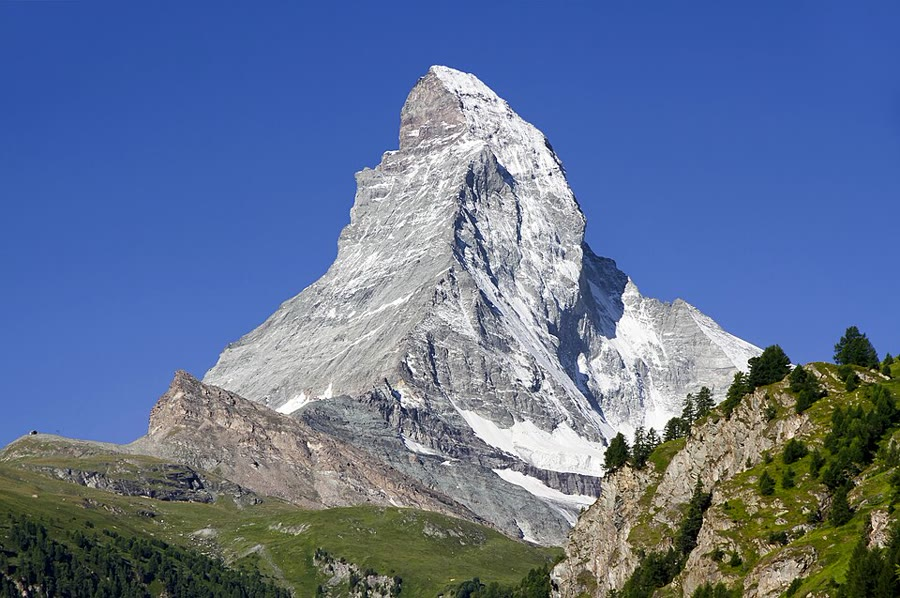
\includegraphics[width=0.7\linewidth]{images/book4/b2-13-matterhorn.jpg}
\par\smallskip{\small त्सेरमाट से देखा गया मैटरहॉर्न (\qty{4478}{m}) का उत्तर-पूर्वी पक्ष:
उसका ऊपरी पिरामिड दाँ ब्लांश अधिक्षेप-तंत्र का अपूलियाई नाइस और गैब्रो है, ऐल्पाइन टेथिस के \omterm{def:b2:alpine-orogen:ophiolite}{ओफ़ियोलाइटों} पर
एक \omterm{def:b2:alpine-orogen:klippe}{क्लिप}। फ़ोटो: Ximonic (Simo Räsänen), CC BY-SA
4.0।}
\end{omfigure}
% ledger: ispra16:cervino

\subsection*{विलगन-तल और दो त्वचाएँ}

\omterm{def:b2:alpine-orogen:nappes}{नैप} और अधिक्षेप-चादरें दुर्बलता की सतहों पर चलती हैं।

\begin{definition}[डेकोलमां]\label{def:b2:alpine-orogen:decollement}
\emph{डेकोलमां}\index{डेकोलमां} कम कोण वाली वह सतह है जिसके अनुदिश चट्टानों का एक
अनुक्रम अपने नीचे की चट्टानों से अलग होकर उन पर सरकता है, और दोनों पक्ष
स्वतंत्र रूप से विरूपित होते हैं; यह प्रायः वाष्पनिक निक्षेप या शेल जैसी किसी दुर्बल परत का अनुसरण करती है।
\end{definition}

\begin{definition}[पतली-त्वचा और मोटी-त्वचा विवर्तनिकी]\label{def:b2:alpine-orogen:skin}
\emph{पतली-त्वचा विवर्तनिकी}\index{पतली-त्वचा विवर्तनिकी} किसी आधारी \omterm{def:b2:alpine-orogen:decollement}{डेकोलमां} के अनुदिश अपने आधारशैल से
अलग हुए अवसादी आवरण का विरूपण है: आवरण वलित और
प्रणोदित होता है जबकि नीचे का आधारशैल अविरूपित रहता है। \emph{मोटी-त्वचा
विवर्तनिकी}\index{मोटी-त्वचा विवर्तनिकी} वह विरूपण है जिसमें आधारशैल सम्मिलित होता है,
और आवरण तथा आधारशैल साथ-साथ उन भ्रंशों पर छोटे होते हैं जो नीचे आधारशैल में कटते हैं।
\end{definition}
% ledger: lanza22:jura

\begin{definition}[वलन--अधिक्षेप पट्टी]\label{def:b2:alpine-orogen:ftb}
\emph{वलन--अधिक्षेप पट्टी}\index{वलन--अधिक्षेप पट्टी} वलनों और अधिक्षेप भ्रंशों की वह पट्टी है
जो किसी \omterm{def:b2:alpine-orogen:orogen}{पर्वतजनक पट्टी} के बाहरी भाग को छोटा करती है और उसकी अग्रभूमि की ओर बढ़ती है; अधिक्षेप
\omterm{def:b2:alpine-orogen:decollement}{डेकोलमां} से परतों में से होकर सीढ़ीनुमा ऊपर चढ़ते हैं, और उनके ऊपर वलन उगते हैं।
\end{definition}

आल्प्स में दोनों त्वचाएँ हैं। हेल्वेटिक \omterm{def:b2:alpine-orogen:nappes}{नैप} एक पतली-त्वचा \omterm{def:b2:alpine-orogen:ftb}{वलन--अधिक्षेप पट्टी} हैं, यानी
निकट यूरोपीय किनारे के मेसोज़ोइक चूना-पत्थर जो अपने आधारशैल से अलग हो गए। उनका आधार
ग्लारुस अधिक्षेप है, जहाँ पर्मियन लाल परतें सीनोज़ोइक \omterm{def:b2:alpine-orogen:foreland}{फ़्लिश} पर स्थित हैं। इसके विपरीत, मायोसीन में
बाह्य पुंजकों के आधारशैल-खंड, यानी छोटा और मोटा हुआ यूरोपीय आधारशैल (आर-पुंजक,
मों ब्लां, बेलडॉन, पेलवू और आर्जेंतेरा पुंजक), अपने आवरण सहित ऊपर
प्रणोदित हुए: मोटी-त्वचा प्रणोदन।
% ledger: schmid04:units, schmid04:skins, herwegh08:glarus, rosenberg21:massifs

जूरा, स्विस मैदान के उत्तर-पश्चिम में कटकों का चाप, पतली त्वचा का क्लासिकी
उदाहरण है। उत्तर मायोसीन और प्लायोसीन में उसका मेसोज़ोइक आवरण एक \omterm{def:b2:alpine-orogen:decollement}{डेकोलमां} के ऊपर
वलित और प्रणोदित हुआ जो दुर्बल मध्य और ऊपरी ट्राइऐसिक वाष्पनिक निक्षेपों में है, जबकि उसके नीचे का आधारशैल,
जो बाह्य पुंजकों से \omterm{def:b2:alpine-orogen:foreland}{मोलास} द्रोणी के नीचे होता हुआ आगे जाता है, सम्मिलित नहीं था: 
क्लासिकी व्याख्या में धक्का दूर के बाह्य पुंजकों से आया। तब से भूकंपविज्ञान ने
एक मोटी-त्वचा अध्याय जोड़ दिया है। 2000 में सें-उर्सान के भूकंपों का स्रोत
एक किलोमीटर से कम गहराई पर था और उनकी क्रियाविधि अधिक्षेप की थी, यानी आवरण में सक्रिय उथला प्रणोदन,
जबकि अन्य अध्ययन नवीनतम प्लायोसीन से पुनःसक्रिय हुए आधारशैल-भ्रंश पाते हैं। क्या
जूरा अब भी अपने आधारशैल से अलग है, इस पर बहस है।
% ledger: lanza22:jura, schmid04:skins

\begin{inthefield}[एक अधिक्षेप-संपर्क को पढ़ना]
पूर्वी स्विट्ज़रलैंड में फ़्लिम्स और वालेनज़ी के बीच ग्लारुस अधिक्षेप चलता है, जो आल्प्स के
सबसे प्रमुख बड़े कम-कोण अधिक्षेपों में से एक है। उसके अनुदिश पर्मियन लाल परतें,
वेरुकानो, सीनोज़ोइक \omterm{def:b2:alpine-orogen:foreland}{फ़्लिश} के ऊपर स्थित हैं, यानी कहीं अधिक पुरानी चट्टानें छोटी उम्र की चट्टानों पर टिकी हैं। उनके बीच
चूना-पत्थर की एक पतली, तीव्र रूप से अपरूपित पट्टी संपर्क बनाती है: लॉखसाइटन चूना-पत्थर, जिस पर कम से कम 30 से
\qty{40}{km} का विस्थापन केंद्रित हुआ। उन्नीसवीं शताब्दी में हाइम ने इस संरचना को दो विशाल
आमने-सामने उलटे वलनों के रूप में पढ़ा; एशर फ़ॉन डेर लिंट ने इसे एक अधिक्षेप के रूप में पढ़ा था, और अधिक्षेप वाली व्याख्या प्रबल रही। ऐसे संपर्क से मिलने वाला भूवैज्ञानिक
तीन बातें जाँचता है: क्या पुरानी चट्टानें छोटी उम्र की चट्टानों पर स्थित हैं, जो कोई साधारण संस्तरण नहीं कर सकता;
क्या दोनों ओर की परतें संपर्क पर कटी हुई हैं; और क्या संपर्क
स्वयं संस्तरण-तल के बजाय अपरूपित, पुनःक्रिस्टलित चट्टान की एक पट्टी है।
\end{inthefield}
% ledger: herwegh08:glarus

\section{अग्रभूमि द्रोणियाँ: फ़्लिश और मोलास}\label{sec:b2:alpine-orogen:foreland}

पर्वत-पट्टी जिस प्लेट पर सवार होती है उस पर भार डालती है, और प्लेट उसके सामने नीचे झुक जाती है।

\begin{definition}[अग्रभूमि द्रोणी; फ़्लिश; मोलास]\label{def:b2:alpine-orogen:foreland}
\emph{अग्रभूमि द्रोणी}\index{अग्रभूमि द्रोणी} एक लंबी अवसादी द्रोणी है जो
किसी \omterm{def:b2:alpine-orogen:orogen}{पर्वतजनक पट्टी} और उसके सामने के स्थिर महाद्वीप के बीच बनती है, जहाँ प्लेट
अधिक्षेप-कील के भार से नीचे झुकती है; यह अधिक्षेप-अग्र के पास सबसे गहरी होती है और स्वयं
क्रमशः अधिक्षेपित होती जाती है। \emph{फ़्लिश}\index{फ़्लिश} ऐसी द्रोणी का गहरे-जल का भराव है,
मुख्यतः बलुआ पत्थर और शेल के गंदलाव-निक्षेप, जो तब जमते हैं जब द्रोणी अल्पपूरित हो।
\emph{मोलास}\index{मोलास} उसका बाद का उथला-समुद्री और महाद्वीपीय भराव है, मुख्यतः
अपरदित होती पट्टी से आए संगुटिकाश्म और बलुआ पत्थर, जो तब जमते हैं जब आपूर्ति
द्रोणी को भर देती है।
\end{definition}
% ledger: sinclair97:trinity, schmid04:foreland, krenmayr99:molasse

यह झुकाव स्थलमंडल का प्रत्यास्थ आनमन है, जिसका विवेचन पुस्तक 5 (स्नातक वर्ष 3) के एक
अध्याय में है; यहाँ केवल द्रोणी पर उसका प्रभाव मायने रखता है। सिंक्लेयर ने पैलियोसीन से ओलिगोसीन आयु की आरंभिक ऐल्पाइन \omterm{def:b2:alpine-orogen:foreland}{अग्रभूमि द्रोणी} का वर्णन
एक ``अल्पपूरित त्रयी'' के रूप में किया: महाद्वीपीय पक्ष पर चूना-पत्थर, बीच में अर्ध-वेलापवर्ती पंक,
और अधिक्षेप-अग्र से सटे गहरे-जल के गंदलाव-निक्षेप। जैसे-जैसे अधिक्षेप आगे बढ़े, द्रोणी
उनके साथ खिसकी: स्विट्ज़रलैंड के आर-पार उसकी महाद्वीपीय तटरेखा 8.5
से \qty{12.9}{mm} प्रति वर्ष की दर से उत्तर-पश्चिम की ओर सरकी, और द्रोणी लगभग स्थिर आकार के साथ कम से कम
\qty{210}{km} यूरोपीय प्लेट के ऊपर स्थानांतरित हुई।
% ledger: sinclair97:trinity

उत्तर ऐल्पाइन \omterm{def:b2:alpine-orogen:foreland}{मोलास} द्रोणी, जो समुद्री आल्प्स से वियना तक फैली है, उत्तर इओसीन में
धँसने लगी। निम्न ओलिगोसीन \omterm{def:b2:alpine-orogen:foreland}{फ़्लिश}, जो अब हेल्वेटिक \omterm{def:b2:alpine-orogen:nappes}{नैपों} के शीर्ष पर मिलता है,
गहरे जल के एक अंतिम चरण को अंकित करता है; उत्तर ओलिगोसीन से उत्तर मायोसीन तक नदियों ने
युवा पर्वतों से महाद्वीपीय बजरी और रेत फैलाई। नाम पुराना है: H.-B. डी सोस्यूर ने
1779 में \emph{\omterm{def:b2:alpine-orogen:foreland}{मोलास}} शब्द चलाया। भराव पट्टी की ओर मोटा होता जाता है:
ऑस्ट्रियाई खंड में अधिक्षेप-अग्र पर \qty{4000}{m} से अधिक तक, और द्रोणी में अन्यत्र
नदी-संगुटिकाश्मों का उत्तर ओलिगोसीन का एक अकेला अनुक्रम लगभग \qty{4}{km} मोटा है। द्रोणी का
दक्षिणी भाग अधिक्षेपित हो चुका है: लगभग \qty{60}{km} चौड़ी ऑस्ट्रियाई बहिर्भाग-पट्टी द्रोणी की पूर्व चौड़ाई के
एक-चौथाई से कम है। अधिक्षेपित \omterm{def:b2:alpine-orogen:foreland}{मोलास} स्वयं अधिक्षेपों में
उप-ऐल्पाइन \omterm{def:b2:alpine-orogen:foreland}{मोलास} के रूप में फँसा है, यानी पट्टी के उत्तरी किनारे के अनुदिश दक्षिण की ओर नत
संगुटिकाश्म की परतें।
% ledger: schmid04:foreland, krenmayr99:molasse, gs18:conglomerates

आल्प्स के दक्षिण में पो मैदान दक्षिणी आल्प्स की कम विरूपित एड्रियाटिक अग्रभूमि पर
स्थित है। उसके सबसे युवा, प्लायोसीन और प्लाइस्टोसीन, अवसाद आंशिक रूप से ऐल्पाइन
संरचनाओं को असंगति के साथ ढकते हैं और आंशिक रूप से दक्षिणी आल्प्स
और एपेनाइन के अंतिम अधिक्षेपों द्वारा विरूपित हैं।
% ledger: schmid04:foreland

\begin{omfigure}
\centering
\begin{tikzpicture}[x=0.5cm, y=0.6cm, font=\scriptsize]
\begin{scope}
\node[anchor=west, font=\scriptsize\bfseries] at (0,2.4) {(क) अल्पपूरित: फ़्लिश};
\fill[blue!8] (0,0) -- (12,0) -- (12,1.4) -- (9.0,1.4) -- (4,0.05) -- (0,0.05) -- cycle;
\fill[gray!25] (0,0) -- (12,-1.1) -- (12,-1.9) -- (0,-0.8) -- cycle;
\fill[omThm!30] (9.0,1.4) -- (12,2.2) -- (12,-1.1) -- (9.5,-0.87) -- cycle;
\fill[green!25!gray!40] (5.5,-0.5) -- (9.5,-0.87) -- (9.3,-0.35) -- (7.0,-0.2) -- cycle;
\node at (10.9,0.6) {कील};
\node at (2,-0.45) {क्रेटॉन};
\node[anchor=north] at (7.3,-0.9) {गंदलाव-निक्षेप};
\draw[->] (7.3,-0.95) -- (7.6,-0.55);
\end{scope}
\begin{scope}[xshift=6.4cm]
\node[anchor=west, font=\scriptsize\bfseries] at (0,2.4) {(ख) अतिपूरित: मोलास};
\fill[gray!25] (0,0) -- (12,-1.1) -- (12,-1.9) -- (0,-0.8) -- cycle;
\fill[omThm!30] (8.5,1.6) -- (12,2.4) -- (12,-1.1) -- (9.0,-0.82) -- cycle;
\fill[yellow!40] (1.5,-0.13) -- (9.0,-0.82) -- (8.5,1.0) -- (5,0.35) -- cycle;
\fill[blue!8] (0,0) -- (1.5,-0.13) -- (5,0.35) -- (4,0.4) -- (0,0.4) -- cycle;
\node at (10.6,0.6) {कील};
\node at (2,-0.45) {क्रेटॉन};
\node at (6.2,-0.05) {बजरी, रेत};
\end{scope}
\end{tikzpicture}
\par\smallskip{\small दो चरणों में एक \omterm{def:b2:alpine-orogen:foreland}{अग्रभूमि द्रोणी} (योजनामूलक)। (क)~आरंभ में झुकी
प्लेट अवसाद के आने से तेज़ी से धँसती है: अधिक्षेप-कील से सटा गहरा जल, जहाँ
गंदलाव-निक्षेप (\omterm{def:b2:alpine-orogen:foreland}{फ़्लिश}) जमा होते हैं। (ख)~बाद में अपरदित होती पट्टी उससे अधिक आपूर्ति करती है जितनी द्रोणी
समा सकती है: नदियाँ उसे बजरी और रेत (\omterm{def:b2:alpine-orogen:foreland}{मोलास}) से भर देती हैं, और कील अपने ही मलबे पर
प्रणोदित होती है।}
\end{omfigure}
% ledger: sinclair97:trinity, schmid04:foreland

\section{इतिहास को पढ़ना: अनुप्रस्थ काटें और भूभौतिकी}\label{sec:b2:alpine-orogen:sections}

मानचित्र बताता है कि इकाइयाँ कहाँ हैं; अनुप्रस्थ काट बताती है कि वे नीचे कैसे पड़ी हैं, और उसकी
जाँच की जा सकती है।

\begin{definition}[संतुलित अनुप्रस्थ काट]\label{def:b2:alpine-orogen:balanced}
\emph{संतुलित अनुप्रस्थ काट}\index{संतुलित अनुप्रस्थ काट} विरूपित चट्टानों की वह अनुप्रस्थ काट है,
जो परिवहन की दिशा के समांतर खींची गई हो और जिसे चट्टान जोड़े या खोए बिना
किसी भूवैज्ञानिक रूप से युक्तिसंगत अविरूपित अवस्था में लौटाया जा सके: काट में चिह्नक परतों की लंबाइयाँ
और शैल इकाइयों के क्षेत्रफल विरूपित और पुनर्स्थापित
अवस्थाओं के बीच संरक्षित रहते हैं।
\end{definition}

पुनर्स्थापन \emph{पिन रेखाओं} पर टिका होता है, यानी काट के सिरों पर परतों के आर-पार खिंची रेखाएँ,
जो वहाँ चुनी जाती हैं जहाँ चट्टानें एक-दूसरे पर से नहीं सरकीं।

\begin{proposition}[रेखा-लंबाई और क्षेत्रफल संतुलन]\label{prop:b2:alpine-orogen:balance}
विरूपित अवस्था में एक-दूसरे से $l$ दूरी पर स्थित दो पिन रेखाओं के बीच, मान लीजिए किसी चिह्नक परत की
परत के अनुदिश मापी गई लंबाई $l_0$ है, और मूल मोटाई $t$ वाले किसी स्तर का
अनुप्रस्थ-काट क्षेत्रफल $A$ है। यदि काट के तल में लंबाई और क्षेत्रफल संरक्षित रहते हैं, तो
\begin{enumerate}
\item विरूपण से पहले परत $l_0$ लंबी थी, लघुकरण
$e = 1 - l/l_0$ है और लघुकरण-दूरी $S = l_0 - l$ है;
\item स्तर की पुनर्स्थापित लंबाई $l_0 = A/t$ है;
\item यदि कोई चिह्नक क्षितिज किसी समतल \omterm{def:b2:alpine-orogen:decollement}{डेकोलमां} के ऊपर $d$ गहराई पर था, तो चिह्नक के मूल स्तर से
ऊपर उठी चट्टान का क्षेत्रफल, उसका \emph{अतिरिक्त क्षेत्रफल} $A_e$, $S\,d$ के बराबर है;
अतः $d = A_e/S$।
\end{enumerate}
\end{proposition}

\begin{omfigure}
\centering
% book's own geometry (figdata/bachelor-2/alps.py)
\begin{tikzpicture}
\begin{axis}[width=0.86\linewidth, height=4.0cm, axis equal image, xmin=-1.5, xmax=31.5,
  ymin=-7.5, ymax=4.8, axis lines=none, clip=false]
\addplot[omThm, line width=1.2pt] table[x=x_km, y=y_km] {figdata/out/bachelor-2-alps-chevron.dat};
\addplot[gray, line width=1.2pt] table[x=x_km, y=y_km] {figdata/out/bachelor-2-alps-chevron0.dat};
\draw[dashed] (axis cs:0,-7) -- (axis cs:0,4.3);
\draw[dashed] (axis cs:22.98,-1.2) -- (axis cs:22.98,4.3);
\draw[dashed] (axis cs:30,-7) -- (axis cs:30,-4.8);
\draw[<->] (axis cs:0,-1.4) -- node[below, font=\scriptsize] {$l = \qty{23.0}{km}$} (axis cs:22.98,-1.4);
\node[font=\scriptsize, anchor=south] at (axis cs:15,-5.9) {पुनर्स्थापित: $l_0 = \qty{30.0}{km}$};
\node[font=\scriptsize, anchor=west] at (axis cs:23.3,2.2) {पार्श्व-नति \qty{40}{\degree}};
\node[font=\scriptsize, anchor=south] at (axis cs:0,4.3) {पिन};
\node[font=\scriptsize, anchor=south] at (axis cs:22.98,4.3) {पिन};
\end{axis}
\end{tikzpicture}
\par\smallskip{\small रेखा-लंबाई संतुलन: शेवरॉन वलनों में वलित एक चिह्नक परत, जिसके पार्श्व
\qty{40}{\degree} पर नत हैं (ऊपर), और वही परत अपनी पिन रेखाओं के बीच पुनर्स्थापित
(नीचे), वास्तविक पैमाने पर। हर पार्श्व अपनी लंबाई बनाए रखता है; वलित परत
$l = 30.0\cos\qty{40}{\degree} = \qty{23.0}{km}$ में फैली है, यानी $1 - \cos\qty{40}{\degree} =
\qty{23.4}{\percent}$ का लघुकरण।}
\end{omfigure}

\begin{proof}
(1) जो परत अपनी लंबाई के अनुदिश न तनती है न सिकुड़ती है, वह अपनी लंबाई बनाए रखती है; लघुकरण
खोई हुई लंबाई का अंश है, जैसा स्कूल में। (2) विरूपण से पहले स्तर लंबाई
$l_0$ और मोटाई $t$ की एक पट्टी है, जिसका क्षेत्रफल $l_0 t$ है, और क्षेत्रफल संरक्षित रहता है। (3) विरूपण से
पहले, चिह्नक के स्तर और \omterm{def:b2:alpine-orogen:decollement}{डेकोलमां} के बीच की चट्टान $l_0$
लंबी और $d$ मोटी एक पट्टी भरती थी। उसके बाद, पिन रेखाओं के बीच, वही चट्टान $l$ लंबी एक पट्टी भरती है,
जो \omterm{def:b2:alpine-orogen:decollement}{डेकोलमां} से चिह्नक के मूल स्तर तक जाती है और जिसका क्षेत्रफल $l\,d$ है, और साथ में उस स्तर से ऊपर धकेला गया अतिरिक्त
क्षेत्रफल। संरक्षण से $l_0 d = l\,d + A_e$ मिलता है, अतः $A_e = (l_0 -
l)\,d = S\,d$। यह संबंध मापे गए अतिरिक्त क्षेत्रफल और लघुकरण से किसी छिपे \omterm{def:b2:alpine-orogen:decollement}{डेकोलमां} की
गहराई देता है।
\end{proof}


\begin{method}[किसी अनुप्रस्थ काट का पुनर्स्थापन]\label{met:b2:alpine-orogen:restore}
\begin{enumerate}
\item परिवहन-दिशा के समांतर एक काट चुनिए, और दो पिन रेखाएँ वहाँ जहाँ
परतों के बीच कोई सरकन नहीं हुई।
\item पिनों के बीच हर चिह्नक परत को उसकी लंबाई के अनुदिश मापिए, और किसी अधिक्षेप द्वारा दोहराया गया
हर भाग भी गिनिए।
\item परतों को उनकी मापी गई लंबाइयों पर समतल बिछाइए, स्तरों का क्रम बनाए रखते हुए,
और पुनर्स्थापित काट पर भ्रंशों को फिर से खींचिए: उनके कट-ऑफ़ बिना रिक्ति
या अतिव्याप्ति के एक सीध में आने चाहिए।
\item तुलना कीजिए: एक ही अधिक्षेप-चादर की परतों की पुनर्स्थापित लंबाई एक-सी होनी चाहिए; स्तरों के
क्षेत्रफल, उनकी मोटाइयों से भाग देने पर, भी वही लंबाइयाँ देने चाहिए। जो काट
विफल हो, वह जैसी खींची गई है वैसी स्वीकार्य नहीं है।
\end{enumerate}
\end{method}

संतुलन किसी काट की जाँच है, उसका प्रमाण नहीं, और उसकी मान्यताएँ मायने रखती हैं। जूरा में
शासराल के पास, जुरैसिक के शीर्ष का रेखा-लंबाई संतुलन \qty{5.1}{km} का
विस्थापन देता है, पर क्षेत्रफल संतुलन और अग्र-प्रतिरूपण \qty{11.3}{km} देते हैं: अतिरिक्त
\qty{6.2}{km} जुरैसिक शेलों में एक दूसरे, ऊपरी विलगन-तल के अनुदिश ले जाया गया और
आगे उत्तर के वलनों को सौंप दिया गया। एक चिह्नक परत आधी गति चूक गई थी। उसी अध्ययन ने
जूरा में प्रचलित दो अन्य व्याख्याओं को तौला, और उनकी आवश्यकता नहीं पाई: वलनों को ऊपर धकेलते
आधारशैल-उभार, और अपनी ओर बहते ट्राइऐसिक वाष्पनिक निक्षेपों से मोटे हुए अपनति-क्रोड, एक ऐसी
प्रक्रिया जो क्षेत्रफल संतुलन को विफल कर देती है, क्योंकि वाष्पनिक स्तर अब अपनी मोटाई
नहीं रखता।
% ledger: schori15:chasseral, schori15:evaporite-flow

\subsection*{कितना लघुकरण?}

पूरे अनुप्रस्थ-पथों पर लागू करने पर संतुलन पट्टी का कुल लघुकरण देता है, और उत्तर
मान्यताओं के साथ बदलते हैं। मध्य आल्प्स के आर-पार, NFP-20 अनुप्रस्थ-पथ के अनुदिश, टक्कर-जनित
लघुकरण के अनुमान पहले के कार्य में लगभग \qty{125}{km}, 2015 के एक संकलन में \qty{160}{km} और
2021 की एक समीक्षा में \qty{144}{km} रहे हैं; पेरिएड्रियाटिक रेखा पर दक्षिणावर्ती सरकन जोड़ने पर, जिसने
अपूलिया को पट्टी के अनुदिश बग़ल में खिसकाया, कुल अभिसरण 206 और
\qty{250}{km} के बीच हो जाता है, इस पर निर्भर करते हुए कि कितनी सरकन मानी जाए। पश्चिमी आल्प्स में अनुमान
124 से \qty{243}{km} तक हैं। इनमें से हर एक पुनर्स्थापित टुकड़ों का योग है, और हर टुकड़े की
अपनी पिन रेखाएँ हैं और इस बारे में अपने अनुमान कि अपरदन और क्षेपण ने क्या हटाया।
% ledger: rosenberg21:shortening

\subsection*{भूभौतिकी क्या देखती है}

गहराई पर काटें भूभौतिकी पर टिकी हैं। पट्टी के आर-पार गहरे भूकंपीय परावर्तन प्रोफ़ाइल
लिए गए हैं (पश्चिमी आल्प्स में एकॉर्स--क्रॉप, स्विट्ज़रलैंड में NFP-20 पश्चिम और पूर्व,
पूर्व में TRANSALP), और भूकंपमापियों के सघन जाल अब मोहो का मानचित्र
ग्राही फलनों (रिसीवर फ़ंक्शन) से बनाते हैं, यानी भूपर्पटी के आधार पर दूरभूकंपी P तरंगों के S तरंगों में रूपांतरणों से।
ऐल्पऐरे मानचित्र, जो एक लाख से अधिक ग्राही फलनों से बना है,
मोहो को पट्टी के चारों ओर लगभग \qty{30}{km} पर पाता है, जो महाद्वीपों के लिए सामान्य है, और आल्प्स के नीचे 55 से
\qty{60}{km} पर; यूरोपीय मोहो उत्तर-पश्चिम में लगभग \qty{30}{km} से पर्वतमाला के नीचे लगभग
\qty{55}{km} तक धीरे-धीरे नत होता है।
नीचे की योजनामूलक काट सार रूप में बताती है कि मध्य आल्प्स के आर-पार NFP-20 प्रोफ़ाइलों को कैसे
पढ़ा जाता है।
% ledger: schmid04:transects, michailos23:moho

\begin{omfigure}
\centering
\begin{tikzpicture}[x=0.6cm, y=0.5cm, font=\scriptsize]
% surface and cover
\fill[yellow!30] (0,0) -- (3.0,0) -- (6.5,-0.3) -- (8.0,0.4) -- (8.0,-0.9) -- (0,-0.6) -- cycle;
\fill[gray!12] (0,-0.6) -- (8.0,-0.9) -- (12.5,-4.5) -- (15,-3.5) -- (16.5,-6.6) -- (16,-8.3)
  -- (0,-5.0) -- cycle;
\fill[gray!35] (0,-5.0) -- (16,-8.3) -- (17.5,-10.0) -- (0,-6.0) -- cycle;
% Helvetic and Aar
\fill[cyan!25] (8.0,0.4) -- (10.0,1.6) -- (11.0,1.2) -- (9.5,-0.4) -- (8.0,-0.9) -- cycle;
\fill[gray!12] (8.0,-0.9) -- (9.5,-0.4) -- (11.0,1.2) -- (12.0,2.0) -- (12.8,0.2) -- (11.5,-1.8)
  -- (12.5,-4.5) -- cycle;
% Penninic stack
\fill[omThm!35] (12.0,2.0) -- (14.5,2.6) -- (17.0,2.2) -- (17.3,-1.0) -- (15.0,-3.5) -- (12.5,-4.5)
  -- (11.5,-1.8) -- (12.8,0.2) -- cycle;
% Austroalpine/Apulia and Southern Alps
\fill[orange!30] (17.0,2.2) -- (19.0,1.6) -- (24,0.2) -- (26,0) -- (26,-3.5) -- (20.5,-4.0)
  -- (17.3,-1.0) -- cycle;
\fill[brown!35] (17.3,-1.0) -- (20.5,-4.0) -- (19.0,-7.0) -- (16.5,-6.6) -- (15,-3.5) -- cycle;
\fill[gray!35] (20.5,-4.0) -- (26,-3.5) -- (26,-6.0) -- (19.0,-7.0) -- cycle;
\fill[yellow!30] (23.5,0.3) -- (26,0) -- (26,-0.5) -- (24.5,-0.3) -- cycle;
\draw[thick] (17.3,-1.0) -- (17.0,2.2);
\draw[thick] (8.0,-0.9) -- (12.5,-4.5);
\draw[dashed] (0,-6.0) -- (17.5,-10.0);
\draw[dashed] (19.0,-7.0) -- (26,-6.0);
\node at (2.2,-0.25) {जूरा};
\node at (5.2,-0.35) {मोलास};
\node at (9.0,0.15) {हेल्वेटिक};
\node at (10.6,-0.6) {आर-पुंजक};
\node at (14.6,0.4) {पेनिनिक नैप};
\node at (21.2,-0.9) {दक्षिणी आल्प्स};
\node at (24.9,-0.3) {पो};
\node at (18.0,-4.8) {इव्रिया};
\node[align=center] at (5,-3.0) {यूरोपीय भूपर्पटी};
\node[anchor=north] at (3.2,-7.4) {यूरोपीय मोहो};
\node at (10,-9.3) {प्रावार};
\node at (23,-7.7) {प्रावार};
\node[anchor=north] at (23,-6.55) {एड्रियाटिक मोहो};
\node[anchor=south, align=center] at (17.2,2.25) {पेरिएड्रियाटिक\\रेखा};
\draw[-{Latex[length=2mm]}] (1.0,0.5) -- (0.0,0.5);
\node[anchor=south] at (0.5,0.5) {उ-प};
\draw[-{Latex[length=2mm]}] (25.0,1.2) -- (26.0,1.2);
\node[anchor=south] at (25.5,1.2) {द-पू};
\end{tikzpicture}
\par\smallskip{\small जूरा से पो मैदान तक मध्य आल्प्स के आर-पार एक योजनामूलक भूपर्पटीय काट
(पैमाने के बिना; श्मिड और सहकर्मियों द्वारा संकलित NFP-20 अनुप्रस्थ-पथों की व्याख्याओं के अनुसार)। यूरोपीय भूपर्पटी,
जिसके शीर्ष से जूरा वलित होकर अलग हुआ है, हेल्वेटिक \omterm{def:b2:alpine-orogen:nappes}{नैपों}, आर-पुंजक और पेनिनिक \omterm{def:b2:alpine-orogen:nappes}{नैप-ढेर} के नीचे
नत होती है; पेरिएड्रियाटिक रेखा के दक्षिण में, इव्रिया पिंड की कील सहित अपूलियाई भूपर्पटी यूरोपीय मोहो के ऊपर
स्थित है, और दक्षिणी आल्प्स पो मैदान पर दक्षिण की ओर
प्रणोदित हैं।}
\end{omfigure}
% ledger: schmid04:transects, schmid04:units, schmid04:apulia, schmid04:skins


\begin{omfigure}
\centering
% ledger: data:b4-etopo-alps, data:b4-alps-moho, michailos23:moho
\begin{tikzpicture}
\begin{groupplot}[group style={group size=1 by 2, vertical sep=0.25cm, x descriptions at=edge bottom},
  width=0.92\linewidth, xmin=0, xmax=300, tick label style={font=\scriptsize},
  label style={font=\small}]
\nextgroupplot[height=3.6cm, ymin=0, ymax=4000, ylabel={ऊँचाई (\unit{m})},
  ytick={0,1000,2000,3000,4000}, y tick label style={/pgf/number format/1000 sep={}},
  legend style={font=\scriptsize, at={(0.99,0.97)}, anchor=north east, draw=none, fill=none}]
\addplot[gray, line width=0.4pt] table[x=km, y=max_m] {figdata/out/bachelor-2-alps-swath.dat};
\addplot[omThm, line width=1pt] table[x=km, y=mean_m] {figdata/out/bachelor-2-alps-swath.dat};
\legend{पट्टी-अधिकतम, पट्टी-माध्य}
\node[font=\scriptsize, anchor=south west] at (axis cs:2,2650) {A (पो मैदान)};
\node[font=\scriptsize, anchor=south east] at (axis cs:298,1500) {B};
\nextgroupplot[height=4.6cm, ymin=0, ymax=70, y dir=reverse, xlabel={\qty{45.3}{\degree} N से उत्तर की ओर,
  \qty{8}{\degree} E के अनुदिश दूरी (\unit{km})}, ylabel={गहराई (\unit{km})},
  legend style={font=\scriptsize, at={(0.99,0.03)}, anchor=south east, draw=none, fill=none}]
\addplot[only marks, mark=*, mark size=1.6pt, black] table[x=km, y=moho_km] {figdata/out/bachelor-2-alps-moho.dat};
\addplot[omThm, dashed, line width=0.8pt] table[x=km, y=airy_km] {figdata/out/bachelor-2-alps-airy.dat};
\addplot[gray, densely dotted] coordinates {(0,30) (300,30)};
\legend{मोहो-चयन, एयरी पूर्वानुमान, \qty{30}{km}}
\end{groupplot}
\end{tikzpicture}
\par\smallskip{\small \qty{8}{\degree} E के अनुदिश प्रोफ़ाइल A--B। ऊपर: याम्योत्तर के दोनों ओर
\qty{0.25}{\degree} की एक पट्टी में ETOPO1 बिंदुओं की माध्य और अधिकतम ऊँचाई।
नीचे: ऐल्पऐरे ग्राही-फलन मानचित्र (मिखाइलोस और सहकर्मी, CC BY 4.0) में इस याम्योत्तर पर चुनी गई मोहो-गहराइयाँ,
और वह मोहो जो स्थानीय एयरी समस्थिति पट्टी-माध्य उच्चावच के नीचे रखती,
\qty{30}{km} भूपर्पटी और घनत्वों 2700 और
\qty{3300}{kg.m^{-3}} के लिए।}
\end{omfigure}

ऊपर का प्रोफ़ाइल इस जड़ की तुलना प्रथम वर्ष वाले
खंड के एयरी प्रतिरूप से करता है। प्रोफ़ाइल के सबसे ऊँचे भाग के नीचे, जहाँ पट्टी-माध्य उच्चावच
\qty{2.74}{km} तक पहुँचता है (\qty{46.5}{\degree} N पर), एक स्थानीय एयरी जड़ मोहो को
$30 + 4.5 \times 2.74 = \qty{42.3}{km}$ पर रखती; वह \qty{36.3}{km} पर प्रेक्षित है। लगभग सौ
किलोमीटर और दक्षिण में, पो मैदान के किनारे पर, जहाँ माध्य उच्चावच केवल
\qty{0.65}{km} है, प्रेक्षित मोहो प्रोफ़ाइल में सबसे गहरा है, \qty{61.2}{km}। जड़ शिखरों के नीचे नहीं है: वह
अपूलिया की ओर विस्थापित है। जिस खंड पर चयन उपलब्ध हैं, वहाँ \qty{30}{km} के नीचे मापा गया
उसका अनुप्रस्थ-काट क्षेत्रफल लगभग \qty{2300}{km^2} है, जबकि ऊपर के उच्चावच की एयरी
जड़ों के लिए यह लगभग \qty{1500}{km^2} है। वर्तमान स्थलाकृति की स्थानीय प्रतिपूर्ति
जड़ की व्याख्या नहीं करती। फ़िफ़्नर और सहकर्मी एक अतिरिक्त भार की ओर इंगित करते हैं: इव्रिया पिंड, यानी पट्टी के भीतर
एड्रियाटिक प्रावार और निचली भूपर्पटी की एक कील, जिसने यूरोपीय प्लेट को नीचे झुकाने में
सहायता की।
% ledger: data:b4-etopo-alps, data:b4-alps-moho, michailos23:moho, pfiffner02:ivrea

गुरुत्व यही कहानी दूसरे ढंग से कहता है। समूचे आल्प्स का बूगेर विसंगति मानचित्र पर्वतमाला के अनुदिश
$-100$ से \qty{-170}{mGal} का एक ऐल्पाइन गुरुत्व-निम्न दिखाता है, जो मध्य
आल्प्स में सबसे गहरा है और मोटी हुई जड़ की हल्की भूपर्पटी से आता है; लगभग $-80$ से
\qty{-140}{mGal} का एक पो द्रोणी निम्न; और, पश्चिमी आल्प्स और पो मैदान के बीच, संकरा इव्रिया गुरुत्व-उच्च,
\qty{+40}{mGal} तक, जहाँ वह सघन निचली भूपर्पटी और प्रावार
सतह के निकट आते हैं।
% ledger: zahorec21:gravity

\section{आल्प्स की एक समयरेखा}\label{sec:b2:alpine-orogen:timeline}

इस अध्याय की तिथियों को एकत्र करने से पट्टी का इतिहास एक तालिका में मिलता है
(नीचे की तालिका)।

\begin{omfigure}
\centering\small
\begin{tabular}{p{0.28\linewidth}|p{0.62\linewidth}}
समय & घटना \\ \hline
मध्य जुरैसिक & पिएमोंट--लिगुरिया महासागर खुलता है; उसके गैब्रो
\qty{164}{Ma} पर क्रिस्टलित होते हैं \\
आरंभिकतम क्रिटेशस & ब्रियांसोनै के उत्तर में वालै महासागर खुलता है \\
लगभग \qty{100}{Ma} & पूर्वी आल्प्स में क्रिटेशस पर्वतजनन का उच्च-दाब शिखर \\
उत्तर क्रिटेशस & अपूलियाई किनारे (सेसिया मंडल) का क्षेपण होता है; महासागर का
अपूलियाई किनारा सक्रिय है \\
48 से \qty{44}{Ma} & त्सेरमाट--सास महासागर-तल अपने सबसे गहरे बिंदु पर पहुँचता है, लागो दी चिन्याना पर कोसाइट और
हीरा \\
मध्य से उत्तर इओसीन & वालै महासागर बंद होता है; \omterm{def:b2:alpine-orogen:foreland}{मोलास} द्रोणी धँसने लगती है \\
\qty{35}{Ma} & डोरा माइरा की महाद्वीपीय भूपर्पटी अति-उच्च दाब पर \\
ओलिगोसीन और मायोसीन & ग्लारुस अधिक्षेप; \omterm{def:b2:alpine-orogen:foreland}{मोलास} बजरी उत्तरी अग्रभूमि को भरती है (उत्तर
ओलिगोसीन से उत्तर मायोसीन) \\
मायोसीन & बाह्य पुंजकों का मोटी-त्वचा उत्थान; दक्षिणी आल्प्स दक्षिण की ओर
प्रणोदित होते हैं \\
उत्तर मायोसीन से प्लायोसीन & जूरा का पतली-त्वचा वलन \\
आज & तलमापन मध्य आल्प्स के क्रोड में \qty{1.3}{mm} प्रति वर्ष तक का सापेक्ष शैल-उत्थान
दिखाता है
\end{tabular}
\par\smallskip{\small ग्यारह चरणों में आल्प्स; स्रोत ऊपर के खंडों में
उद्धृत हैं।}
\end{omfigure}
% ledger: schmid04:alpine-tethys, rubatto98:zsf, schmid04:two-orogenies, halama20:cignana, schmid04:foreland, rh01:exhumation, herwegh08:glarus, schmid04:skins, schmid04:apulia, champagnac09:uplift

अंतिम पंक्ति अभिसरण का अंत नहीं है। मध्य आल्प्स के आर-पार बार-बार किया गया तलमापन
जूरा के उत्तर में लगभग \qty{-0.4}{mm} प्रति वर्ष से लेकर पर्वतमाला के क्रोड में
\qty{1.3}{mm} प्रति वर्ष तक का सापेक्ष शैल-उत्थान देता है, जबकि GPS मापन संकेत देते हैं कि
मध्य आल्प्स आज अभिसरित नहीं हो रहे। शांपान्याक और सहकर्मी इस उत्थान को अपरदन द्वारा भार-मुक्त की जा रही
भूपर्पटी का समस्थितिक प्रतिक्षेप मानते हैं: पर्वत इसलिए उठते हैं क्योंकि वे घिसते जाते हैं।
% ledger: champagnac09:uplift

\section*{अभ्यास}\label{sec:b2:alpine-orogen:exercises}

अभ्यासों के लिए आँकड़े: $g = \qty{9.8}{m.s^{-2}}$,
$G = \qty{6.674e-11}{m^3.kg^{-1}.s^{-2}}$।

\begin{exercise}[$\star$]\label{exo:b2:alpine-orogen:1}
किसी अनुप्रस्थ काट में, दो पिन रेखाओं के बीच अपने वलनों के अनुदिश मापी गई एक चूना-पत्थर परत
\qty{36.0}{km} लंबी है; पिन रेखाएँ \qty{27.0}{km} दूर हैं। (क)
\cref{prop:b2:alpine-orogen:balance} का उपयोग करके लघुकरण $e$ और लघुकरण-दूरी
$S$ निकालिए। (ख) उत्तर के सही होने के लिए परत के बारे में क्या सत्य होना चाहिए?
\end{exercise}

\begin{exercise}[$\star$]\label{exo:b2:alpine-orogen:2}
किसी भूवैज्ञानिक मानचित्र पर, (क) नाइस का \qty{4}{km} लंबा एक अंडाकार धब्बा जुरैसिक
चूना-पत्थर पर स्थित है, जिसकी सीमा एक अधिक्षेप है जो चारों ओर भीतर की ओर, नाइस के नीचे, नत है; (ख)
क्रिटेशस शेल का एक लंबा क्षेत्र नाइस से घिरा है, एक ऐसे अधिक्षेप के अनुदिश जो
चारों ओर बाहर की ओर, नाइस के नीचे, नत है। प्रत्येक संरचना का नाम बताइए और कहिए कि हर स्थिति में
अपरदन ने क्या किया है।
\end{exercise}

\begin{exercise}[$\star$]\label{exo:b2:alpine-orogen:3}
(क) \omterm{def:b2:alpine-orogen:ophiolite}{पेनरोज़ ओफ़ियोलाइट अनुक्रम} की चार इकाइयाँ नीचे से ऊपर के क्रम में लिखिए, और हर एक का मिलान
महासागरीय भूपर्पटी या प्रावार की किसी परत से कीजिए। (ख) शनाये \omterm{def:b2:alpine-orogen:ophiolite}{ओफ़ियोलाइट} में अनावृत
प्रावार, गैब्रो और तकिया बेसाल्ट दिखते हैं, और कोई अवसादी आवरण नहीं। यह सूची पेनरोज़ की
कौन-सी इकाई छोड़ देती है? (ग) \omterm{def:b2:alpine-orogen:ophiolite}{ओफ़ियोलाइट} चौड़े महासागरों के तल का उचित नमूना
क्यों नहीं देते?
\end{exercise}
% ledger: coleman84:penrose, coleman84:settings, corno23:chenaillet

\begin{exercise}[$\star$]\label{exo:b2:alpine-orogen:4}
दक्षिण से मैटरहॉर्न पर चढ़ते हुए एक पर्वतारोही क्रम से मोंते रोसा और
ग्रां सें बर्नार \omterm{def:b2:alpine-orogen:nappes}{नैपों}, त्सेरमाट--सास \omterm{def:b2:alpine-orogen:ophiolite}{ओफ़ियोलाइटों}, कॉम्बैं मंडल और
दाँ ब्लांश अधिक्षेप-तंत्र के नाइसों को पार करता है। (क) हर एक का उद्गम-क्षेत्र बताइए। (ख) क्षेपण के दौरान
कौन-सी प्लेट ऊपरी प्लेट थी? (ग) \omterm{def:b2:alpine-orogen:nappes}{नैप-ढेर} में यह क्रम एक सामान्य नियम क्यों है,
और इसे क्या तोड़ सकता है?
\end{exercise}
% ledger: ispra16:cervino, schmid04:units

\begin{exercise}[$\star\star$]\label{exo:b2:alpine-orogen:5}
मध्य आल्प्स पर लगभग \qty{-170}{mGal} की बूगेर विसंगति है। (क) प्रथम वर्ष वाले
खंड की बूगेर पट्टी, $\Delta g = 2\pi G\,\Delta\rho\,h$, का उपयोग करके वह मोटाई $h$ निकालिए जो
घनत्व-न्यूनता $\Delta\rho = \qty{500}{kg.m^{-3}}$ (प्रावार का स्थान लेती भूपर्पटी) वाली किसी अनंत पट्टी को
यह विसंगति देती है। (ख) ग्राही फलन लगभग \qty{25}{km} की एक जड़ दिखाते हैं, जो
\qty{30}{km} भूपर्पटी के नीचे है। उतनी मोटी अनंत पट्टी कितनी विसंगति देगी? (ग)
प्रेक्षित विसंगति छोटी क्यों है?
\end{exercise}
% ledger: zahorec21:gravity, michailos23:moho

\begin{exercise}[$\star\star$]\label{exo:b2:alpine-orogen:6}
त्सेरमाट--सास \omterm{def:b2:alpine-orogen:ophiolite}{ओफ़ियोलाइट} के गैब्रो \qty{164}{Ma} पर क्रिस्टलित हुए; \omterm{def:b2:alpine-orogen:ophiolite}{ओफ़ियोलाइट}
\qty{44}{Ma} पर, \qty{2.8}{GPa} पर, अपने सबसे गहरे बिंदु पर पहुँचा। (क) क्षेपण के समय महासागरीय
स्थलमंडल कितना पुराना था? (ख) दाब को गहराई में बदलिए, पहले \qty{3000}{kg.m^{-3}} के माध्य
अधिभार-घनत्व से, फिर \qty{3300}{kg.m^{-3}} से। (ग) इस चट्टान के लिए उद्धृत
``\qty{90}{km} से अधिक'' से तुलना कीजिए।
\end{exercise}
% ledger: rubatto98:zsf, halama20:cignana

\begin{exercise}[$\star\star$]\label{exo:b2:alpine-orogen:7}
एक परत ऐसे शेवरॉन वलनों में वलित है जिनके सीधे पार्श्व सभी कोण $\theta$ पर नत हैं।
(क) दिखाइए कि लघुकरण $e = 1 - \cos\theta$ है। (ख) कितनी पार्श्व-नति
\qty{30}{\percent} लघुकरण देती है? (ग) \qty{40}{\degree} और \qty{60}{\degree} पर नत पार्श्व
कितना लघुकरण देते हैं? पहले की जाँच संतुलन वाले खंड के शेवरॉन चित्र से कीजिए।
\end{exercise}

\begin{exercise}[$\star\star$]\label{exo:b2:alpine-orogen:8}
\qty{2.0}{km} मोटा एक आवरण एक समतल \omterm{def:b2:alpine-orogen:decollement}{डेकोलमां} के ऊपर वलित और अधिक्षेपित है। अब
\qty{42}{km} दूर स्थित पिन रेखाओं के बीच उसका अनुप्रस्थ-काट क्षेत्रफल \qty{118}{km^2} है। (क) उसकी पुनर्स्थापित
लंबाई, $S$ और $e$ निकालिए। (ख) अतिरिक्त क्षेत्रफल और आवरण के मूल शीर्ष के नीचे
\omterm{def:b2:alpine-orogen:decollement}{डेकोलमां} की गहराई की गणना कीजिए। (ग) क्या परिणाम संगत है?
\end{exercise}

\begin{exercise}[$\star\star$]\label{exo:b2:alpine-orogen:9}
इस अध्याय के \qty{8}{\degree} E प्रोफ़ाइल के अनुदिश, पट्टी-माध्य ऊँचाई
\qty{2.74}{km} है (\qty{46.5}{\degree} N पर), जहाँ मोहो \qty{36.3}{km} पर चुना गया है, और
\qty{0.65}{km} है (\qty{45.55}{\degree} N पर), जहाँ वह \qty{61.2}{km} पर चुना गया है। (क)
\qty{30}{km} संदर्भ भूपर्पटी, $\rho_c = \qty{2700}{kg.m^{-3}}$ और $\rho_m =
\qty{3300}{kg.m^{-3}}$ के साथ दोनों स्थानों पर एयरी मोहो-गहराई निकालिए। (ख) चयनों से तुलना कीजिए।
(ग) यह तुलना ऐल्पाइन जड़ के टिके रहने के ढंग के बारे में क्या बताती है?
\end{exercise}
% ledger: data:b4-etopo-alps, data:b4-alps-moho, pfiffner02:ivrea

\begin{exercise}[$\star\star\star$]\label{exo:b2:alpine-orogen:10}
जूरा की शासराल काट में, जुरैसिक के शीर्ष का रेखा-लंबाई संतुलन
\qty{5.1}{km} का विस्थापन देता है; क्षेत्रफल संतुलन और प्रतिरूपण \qty{11.3}{km} देते हैं, जिसमें से
\qty{6.2}{km} मध्य जुरैसिक शेलों में एक ऊपरी विलगन-तल के अनुदिश ले जाया गया।
(क) शीर्ष-जुरैसिक परत ने विस्थापन का कितना अंश अंकित किया? (ख) दिखाइए कि
संख्याएँ मेल खाती हैं, और समझाइए कि ऊपरी परत गति का एक भाग क्यों चूक जाती है। (ग) एक अकेली चिह्नक परत से
संतुलन के लिए इससे कौन-सी सामान्य सीख मिलती है?
\end{exercise}
% ledger: schori15:chasseral

\begin{exercise}[$\star\star\star$]\label{exo:b2:alpine-orogen:11}
मध्य आल्प्स के आर-पार लगभग \qty{200}{km} उत्तर-दिष्ट लघुकरण का
अनुमान लगाया गया है, और पेरिएड्रियाटिक रेखा पर लगभग \qty{100}{km} का पूर्व--पश्चिम दक्षिणावर्ती विस्थापन है,
शायद 50, शायद 150। (क) दोनों को लंबवत सदिशों की तरह जोड़िए और
हर विस्थापन के लिए कुल अभिसरण बताइए। (ख) \qty{100}{km} के विस्थापन के लिए अभिसरण
उत्तर--दक्षिण दिशा से कितना कोण बनाता है? (ग) विस्थापन का चुनाव
लघुकरण के तीसरे सार्थक अंक से अधिक क्यों मायने रखता है?
\end{exercise}
% ledger: rosenberg21:shortening

\begin{exercise}[$\star\star\star$]\label{exo:b2:alpine-orogen:12}
ऐल्पाइन \omterm{def:b2:alpine-orogen:foreland}{अग्रभूमि द्रोणी} का स्विस भाग यूरोप के ऊपर कम से कम \qty{210}{km} उत्तर-पश्चिम की ओर
स्थानांतरित हुआ, और उसकी तटरेखा 8.5 से \qty{12.9}{mm} प्रति वर्ष की दर से आगे बढ़ी। (क) यह स्थानांतरण कितने
समय तक चला (अवधियों का परास बताइए)? (ख) ऑस्ट्रियाई खंड में, लगभग
\qty{60}{km} चौड़ी वर्तमान बहिर्भाग-पट्टी द्रोणी की पूर्व चौड़ाई के एक-चौथाई से कम है। न्यूनतम
पूर्व चौड़ाई कितनी थी, और द्रोणी का कितना भाग अधिक्षेपों के नीचे छिपा है? (ग) कोई
\omterm{def:b2:alpine-orogen:foreland}{अग्रभूमि द्रोणी} कभी पूरी तरह संरक्षित क्यों नहीं रह सकती?
\end{exercise}
% ledger: sinclair97:trinity, krenmayr99:molasse

\begin{problem}[{सप्ताहांत समस्या --- काट का पुनर्स्थापन}]\label{pb:b2:alpine-orogen:1}
एक ऐल्पाइन-प्रकार की \omterm{def:b2:alpine-orogen:orogen}{पर्वतजनक पट्टी} को एक प्रतिरूप काट काटती है (एक कल्पित ज्यामिति, पुस्तक की अपनी,
प्रतिरूप के रूप में चिह्नित), जो अग्रभूमि से दूर वाले पक्ष तक पाँच क्षेत्रों से बनी है:
एक अग्रभूमि \omterm{def:b2:alpine-orogen:ftb}{वलन--अधिक्षेप पट्टी}, आज \qty{48}{km} चौड़ी; एक बाह्य \omterm{def:b2:alpine-orogen:nappes}{नैप-ढेर}, \qty{15}{km};
एक आधारशैल पुंजक, \qty{22}{km}; महाद्वीपीय \omterm{def:b2:alpine-orogen:nappes}{नैपों} और \omterm{def:b2:alpine-orogen:ophiolite}{ओफ़ियोलाइटों} का एक आंतरिक मंडल,
\qty{20}{km}; और एक दक्षिण-अभिमुख प्रति-कील, \qty{48}{km}
(नीचे का चित्र)। पूरे समय लंबाइयाँ किलोमीटर में हैं।

\begin{omfigure}
\centering
\begin{tikzpicture}[x=0.075cm, y=0.5cm, font=\scriptsize]
\fill[yellow!30] (0,0) rectangle (48,1);
\fill[cyan!25] (48,0) rectangle (63,1);
\fill[gray!25] (63,0) rectangle (85,1);
\fill[omThm!35] (85,0) rectangle (105,1);
\fill[orange!30] (105,0) rectangle (153,1);
\draw (0,0) rectangle (153,1);
\foreach \x in {48,63,85,105} \draw (\x,0) -- (\x,1);
\node at (24,0.5) {अग्रभूमि पट्टी};
\node[align=center] at (55.5,1.6) {नैप};
\node at (74,0.5) {पुंजक};
\node[align=center] at (95,1.6) {आंतरिक};
\node at (129,0.5) {प्रति-कील};
\node[anchor=north] at (24,0) {48}; \node[anchor=north] at (55.5,0) {15};
\node[anchor=north] at (74,0) {22}; \node[anchor=north] at (95,0) {20};
\node[anchor=north] at (129,0) {48};
\end{tikzpicture}
\par\smallskip{\small सप्ताहांत समस्या की प्रतिरूप काट: उसके पाँच क्षेत्रों की वर्तमान
चौड़ाइयाँ, किलोमीटर में (कुल 153; एक कल्पित ज्यामिति)।}
\end{omfigure}

\noindent\textbf{भाग I --- अग्रभूमि पट्टी का रेखा-लंबाई संतुलन।} उसकी दो पिन
रेखाओं के बीच, जो \qty{48.0}{km} दूर हैं, मुख्य चूना-पत्थर का शीर्ष दस सीधे खंडों से बना है
(क्षैतिज विस्तार $\Delta x$, नति), अग्रभूमि से गिने गए; इसके अतिरिक्त, एक अधिक्षेप-चादर
उसी परत का \qty{6.0}{km} लंबा एक समतल हिस्सा ढकती है, जो उसके नीचे दोहराया गया है।

\smallskip
\begin{center}\small
\begin{tabular}{l|cccccccccc}
खंड & 1 & 2 & 3 & 4 & 5 & 6 & 7 & 8 & 9 & 10\\ \hline
$\Delta x$ (\unit{km}) & 8.0 & 3.0 & 3.0 & 5.0 & 2.5 & 2.5 & 6.0 & 4.0 & 4.0 & 10.0\\
नति (\unit{\degree}) & 0 & 35 & 35 & 0 & 50 & 50 & 10 & 40 & 40 & 5
\end{tabular}
\end{center}
\smallskip

\begin{enumerate}
\item खंड 2, 5 और 8 की परत के अनुदिश लंबाई निकालिए।
\item दोहराए गए हिस्से सहित, पिन रेखाओं के बीच परत की कुल लंबाई
निकालिए।
\item अधिक्षेप-चादर के नीचे छिपे हिस्से को क्यों गिनना ही चाहिए?
\item अग्रभूमि पट्टी का लघुकरण $e$ और लघुकरण-दूरी $S$ निकालिए।
\item उसी तरह मापा गया चूना-पत्थर का आधार \qty{60.2}{km} लंबा है। दोनों परतें कितने से,
और कितने प्रतिशत से, असहमत हैं? क्या काट स्वीकार्य है?
\item आधार के लिए \qty{54.0}{km} की लंबाई का क्या अर्थ होता?
\end{enumerate}

\noindent\textbf{भाग II --- क्षेत्रफल संतुलन और डेकोलमां।} \omterm{def:b2:alpine-orogen:decollement}{डेकोलमां} और
चूना-पत्थर के शीर्ष के बीच का आवरण विरूपण से पहले \qty{2.4}{km} मोटा था; पिन रेखाओं के बीच उसका
क्षेत्रफल \qty{146}{km^2} मापा गया है।
\begin{enumerate}[resume]
\item आवरण की पुनर्स्थापित लंबाई उसके क्षेत्रफल से निकालिए।
\item प्रश्न~2 के रेखा-लंबाई परिणाम से तुलना कीजिए।
\item आवरण के मूल शीर्ष से ऊपर उठा अतिरिक्त क्षेत्रफल निकालिए।
\item उस स्तर के नीचे \omterm{def:b2:alpine-orogen:decollement}{डेकोलमां} की गहराई निगमित कीजिए, और उसकी तुलना आवरण की
मोटाई से कीजिए।
\item यदि क्षेत्रफल \qty{160}{km^2} होता, तो वह कितनी पुनर्स्थापित लंबाई देता? जूरा के संदर्भ में
नामित कौन-सी प्रक्रिया क्षेत्रफल और रेखा-लंबाई में इस प्रकार असहमति ला सकती है?
\item यह पट्टी पतली-त्वचा क्यों है, और उसके नीचे आधारशैल का शीर्ष
कैसा दिखना चाहिए?
\end{enumerate}

\noindent\textbf{भाग III --- बाह्य नैप और उनकी गति।} तीनों बाह्य \omterm{def:b2:alpine-orogen:nappes}{नैपों} की
चिह्नक परत 22, 18 और \qty{25}{km} तक पुनर्स्थापित होती है; ढेर अब
\qty{15}{km} में फैला है। आधारशैल पुंजक में आधारशैल का शीर्ष \qty{30}{km} तक पुनर्स्थापित होता है,
जबकि आज वह \qty{22}{km} है। अग्रभूमि पट्टी 11 और \qty{4}{Ma} के बीच विरूपित हुई,
\omterm{def:b2:alpine-orogen:nappes}{नैप} 30 और \qty{20}{Ma} के बीच।
\begin{enumerate}[resume]
\item \omterm{def:b2:alpine-orogen:nappes}{नैप-ढेर} की पुनर्स्थापित लंबाई और उसकी लघुकरण-दूरी निकालिए।
\item उसका लघुकरण $e$ निकालिए और उसकी तुलना अग्रभूमि पट्टी के लघुकरण से कीजिए।
\item आधारशैल पुंजक का लघुकरण निकालिए। यह किस प्रकार की विवर्तनिकी है?
\item अग्रभूमि पट्टी और \omterm{def:b2:alpine-orogen:nappes}{नैपों} की माध्य लघुकरण-दरें, मिलीमीटर प्रति
वर्ष में, निकालिए।
\item विरूपण काट में से किस दिशा में स्थानांतरित हुआ? क्या यह आल्प्स का
क्रम है?
\item तीनों बाह्य क्षेत्रों का लघुकरण जोड़िए।
\end{enumerate}

\noindent\textbf{भाग IV --- आंतरिक मंडल, महासागर और पूरी काट।}
आंतरिक मंडल में ओफ़ियोलाइट-पट्टियाँ \qty{18}{km} तक पुनर्स्थापित होती हैं। मान लीजिए कि महासागर का
85 से \qty{45}{Ma} तक \qty{0.5}{cm} प्रति वर्ष की माध्य दर से क्षेपण हुआ। आंतरिक मंडल के महाद्वीपीय
\omterm{def:b2:alpine-orogen:nappes}{नैप} \qty{60}{km} तक पुनर्स्थापित होते हैं (आज \qty{20}{km}), और
प्रति-कील की चिह्नक परत \qty{70}{km} तक (आज \qty{48}{km})।
\begin{enumerate}[resume]
\item महासागरीय स्थलमंडल की कितनी लंबाई का क्षेपण हुआ?
\item महासागर की न्यूनतम चौड़ाई बताइए।
\item यह केवल न्यूनतम क्यों है?
\item आंतरिक मंडल और प्रति-कील का लघुकरण निकालिए।
\item पाँचों क्षेत्रों का टक्कर-जनित लघुकरण जोड़िए, और उसकी तुलना इस अध्याय में
मध्य आल्प्स के अनुमानों से कीजिए।
\item भूपर्पटीय जाँच: \qty{30}{km} भूपर्पटी के साथ काट को उसकी पूरी चौड़ाई तक पुनर्स्थापित कीजिए, और
भूपर्पटीय क्षेत्रफल की तुलना आज के क्षेत्रफल से कीजिए,
यानी \qty{45}{km} का माध्य, वर्तमान \qty{153}{km} पर।
वर्तमान काट से भूपर्पटी का कितना अंश ग़ायब है, और वह कहाँ
गई? पूरी काट पर कुल टक्कर-जनित लघुकरण, किलोमीटर तक पूर्णांकित, बताइए।
\end{enumerate}
\end{problem}
